%%This is a very basic article template.
%%There is just one section and two subsections.
\documentclass{article}

\usepackage{amsmath}
\usepackage{amscd}
\usepackage{amssymb}
\usepackage{amsfonts} 
\usepackage{amsthm}
\usepackage{amsfonts}
\usepackage{amsthm}

\usepackage{circuitikz}
\usepackage{pgf}
\usepackage{tikz}
\usetikzlibrary{arrows,snakes,backgrounds}
% \usetikz
\usepackage{subfig}

\usepackage{algpseudocode}
\usepackage{algorithm}

\usepackage[super]{nth}
% \usepackage{appendix}
% \usepackage{listings}
% \usepackage{color}

\usepackage{hyperref}
%\usepackage{url}

\usepackage{cleveref}
\usepackage{cancel}

\usepackage{aviolov_style}
\usepackage{local_style}


\newtheorem{thm}{Theorem}[section]
\newtheorem{lemma}{Theorem}[thm]
% \theoremstyle{definition}
\newtheorem{ex}{Example}[thm]
\newtheorem{defn}{Definition}[thm]

\begin{document}


\title{Stochastic Optimal Control - with a view towards spike control in neurons
\\
{\small Advanced Comprehensive Exam in Mathematics}
\\
{\small Dept. of Math - University of Ottawa}
}
\author{Alexandre Iolov 
$<$\href{mailto:aiolo040@uottawa.ca}
		{aiolo040 at uottawa dot ca}$>$}

\date{January 10, 2013}

\maketitle

\abstract{We review main concepts from stochastic optimal control theory,
including stochastic differential equations, dynamic programing and Pontryagin's
Maximum Principle. We then discuss an optimal control problem in a simple
mathematical model of a neuron where the feedback is minimal and we have a
quasi-open-loop control which necessitates the use of a Maximum Principle for
the system's transition density.}

\tableofcontents

\section{Overview}
Stochastic Optimal Control in continuous time deals with finding
the input which optimizes the performance of a continuous-time dynamical systems
that contain a significant random component in their evolutions.

Here we present a brief overview of the subject starting from the basic notions
of Stochastic Differential Equations (SDEs), 
and then introducing the main tools of Optimal Control, namely the
Hamilton-Jacobi-Bellman equation of Dynamic Programming and the state-adjoint
equations arising from Pontryagin's Maximum Principle. We will not state
proofs, although we sometimes provide heuristic derivations of the main
results.

If I had to learn the material all over again, I would proceed my readings as
follows: First I would read the online notes by Evans on both
SDEs,\cite{Evansa}, and Optimal Control, \cite{Evansb}. I would then read
Jacobs' book, \cite{Jacobs}, especially for the chapter on the Fokker-Planck
equation (ch 7) and then Oksendal \cite{Oksendal2007} for a
more thorough mathematical treatment of SDEs. Having familiarized myself with SDE's I would
return to Optimal Control in the Deterministic Case, starting with \cite{Kirk2004} for the
finite dimensional deterministic case (ODEs) and then \cite{Fleming1975} for the
extension to the stochastic case. I would keep the following for reference \cite{Krylov2008},
\cite{Hanson2007} and finally \cite{Fattorini1999} for the
deterministic infinite-dimensional (PDEs) case.

I have not used any particularly sophisticated numerical
methods, but, for example, Hanson \cite{Hanson2007} discusses both the
Euler-Maruyama scheme for simulating SDEs and the Crank-Nicholson Method for
solving PDEs which is all I have used in my codes.

All of the theoretical results presented in the sequel will be from
the above references. 

\section{Stochastic Differential Equations}
In view of our ultimate goals, we will restrict ourselves to  stochastic
processes whose sample paths have continuous paths, i.e.\ to SDEs driven by
Brownian motion. 

Since the reader is more likely well familiar with the material in this section,
we will not provide proofs, but only state the results with a view towards
establishing the notation for the sequel.

We will assume that the reader is familiar with the following concepts:
\begin{itemize} 
  \item a probability space, $\{\O, \sAlg, P\}$ consisting of a
  probability space, a sigma-algebra and a probability measure
  \item a continuous-time stochastic process, $X_t$
  \item a filtration $\Fil(t)$ and in particular the filtration generated by a
  stochastic process.
\end{itemize}

\subsection{The Wiener Process and the Ito Integral}
The Wiener Process is the fundamental building block of the stochastic calculus,
it is often called Brownian Motion and we will denote it $\{W_t\}_{t\geq 0}$. It
satisfies:
\begin{defn}Wiener Process, $W_t$:
\begin{enumerate}
  \item $W_0 = 0$
  \item $W_t - W_s = N(0, |t-s|)$ , i.e. normally distributed with mean 0,
  variance $|t-s|$)
  \item $\forall \{t_i\}_1^N, \quad \{W_{t_i} - W_{t_{i-1}} \}_2^N \sim$
  independent, i.e $W_t$ has independent increments
\end{enumerate}
\end{defn}
The fact that the finite incremental distributions suffice to specify a unique
continuous-time stochastic process is known as Kolmogorov's extension theorem.
\begin{ex}[from \cite{Evansa} \#21.] Inverted Wiener Process:
\\
Let $W_t$ be a 1-d Wiener Process and define:
\def \Wbar {{\bar{W} }}
\begin{equation*}
\Wbar(t) := \begin{cases}
t W(1/t) & t >0
\\
0 & t = 0
\end{cases}
\end{equation*}
Show $\Wbar(t)- \Wbar(s) \sim N(0, t-s)$.

\begin{proof}[Soln]
\begin{align*}
\Wbar(t) - \Wbar(s) =& t W(1/t) - s W(1/s), \, t>s
\\
=& (t-s)W(1/t) + s W(1/t) - sW(1/s) & \text{recall:} 1/s > 1/t
\\
=& (t-s)N(0, 1/t) - sN(0, 1/s -1/t) & \text{by indnt increments}
\\
=& N\left(0, \frac{(t-s)^2}t + \frac{s^2 }{ 1/s -1/t} \right) & \text{
addition of indnt normal RVs.}
\end{align*}
With some algebra, the variance in the last expression reduces to $t-s$
\end{proof}
\end{ex}

Now, we collect a few more relevant properties of $W_t$:
\begin{enumerate}
  \item The sample paths $W_{[0,\infty)}(\o)$
are almost surely (a.s.) continuous and are in fact Holder continuous for any
exponent $\g < 1/2$
\item The sample paths $W_{[0,\infty)}(\o)$ are nowhere differentiable
\item $W_t$ is a Markov process: $\Prob[W_t \in B | \s(W_{s' \leq s })] =
\Prob[W_t \in B \,| \,W_s]$, for any Borel set, $B \subset \R$, where $\s(W_{s'
\leq s })$ is the filtration generated by the $W_t$
\end{enumerate}



We now turn to defining stochastic integrals based on the Wiener Process.
 
\begin{defn} Progressively Measurable Functions:

Let $\Fil_t$ be the filtration generated by the Wiener Process.

Let $X_t$ be a stochastic process which is $\Fil_t$-measurable $\forall t$ and
which is jointly measurable in $(t,\o)$. We call such an $X_t$
\emph{progressively measurable}
\end{defn}

\begin{defn} $\Ltwopm, \Lonepm$

We define $\Ltwopm[0,T]$ as the space of all progressively measurable
$X$ such that
\begin{equation*}
\Exp \left[ \int_{[0,T]} X_t^2 \intd{t} \right] < \infty
\end{equation*}

Similarly, we define $\Lonepm[0,T]$ as the space of all progressively measurable
$X$ such that
\begin{equation*}
\Exp \left[ \int_{[0,T]} X_t \intd{t} \right] < \infty
\end{equation*} 
\end{defn}

$\Ltwopm$ will be the class of functions for which the Ito integral is
well-defined. 
\begin{defn} Ito Integral:
\label{defn:ito_integral}

Let $P^n := {a = t^n_1 \ldots t^n_{m_n} = b}$ be a partition of the interval
$[a,b] \subset [0, \infty)$. Let $|P_n| = \sup_i|t_i - t_{i-1}|$. 
Take $|P_n| \rightarrow_n 0 $ and consider an $ X_t \in \Ltwopm[a,b]$,

then
\begin{equation}
\int_{[a,b]} X_t \intd{W} := \lim_{n \rightarrow \infty}  
\sum_{i=1}^{m_n} X_{t_i}\left( W(t_{i+1}) - W(t_{i})\right)
\end{equation}

\end{defn}

To be precise, our definition is actually a theorem, and the real
definition is one that uses step functions and passes to the limit.  Also we
will write the limits of integration $\int_0^T \cdot  \intd{W}$ or $\int_{[0,T]}
\cdot  \intd{W}$ interchangeably.
% To justify def'n \ref{defn:ito_integral}, we recall:
% \begin{lemma}[Quadratic Variation]
% \begin{equation}
% \lim_{n \rightarrow \infty} \sum_{i=1}^{m_n} \left( W(t_i) - W(t_{i-1})\right)^2
% = b-a \quad \text{in }  L^2(\O)
% \end{equation}
% \end{lemma}
% The above can be read, heuristically as $\lim \sum (\Delta W)^2 \rightarrow \sum
% \Delta t$, which is the meaning behind the colloquial $\intd{W} =
% \sqrt{dt}$.

Again, we state without proof a few interesting properties of $\int X \intd{W}$:
\begin{thm} Ito Integral Properties

\begin{enumerate}
  \item $\Exp[\int_0^T X \intd{W} ] = 0$ 
  \item $\Exp[\left(\int_0^T X \intd{W}\right)^2 ] = \Exp[\int_0^T X^2
  \intd{t}]$
  \item $I(t) = \int_0^t X \intd{W} $ is a martingale 
  \item $I(t) = \int_0^t X \intd{W} $ has continuous sample paths
\end{enumerate}
\end{thm}

\subsection{Ito SDEs and Ito's Lemma}
\begin{defn} an Ito SDE:

We write
\begin{equation}
dX_t = Fdt + G dW
\end{equation}
on $0 \leq t \leq T$, if $X$ is a real-valued stochastic process satisfying:
\begin{equation*}
X(r) = X(s) + \int_{[s,r]} F \intd{t} + \int_{[s,r]} G \intd{W}
\quad 0\leq s \leq r \leq T
\end{equation*}
for some $F \in \Lonepm[0,T]$ and $G \in \Ltwopm[0,T]$
\end{defn}

We are now ready to present the celebrated Ito Lemma which is the chain-rule of
stochastic calculus:

\begin{thm}[Ito Lemma] Suppose $X$ satisfies the stochastic differential $dX_t =
Fdt + G dW$ as above and take $u(x,t) \in C^{2,1}[ \R \times [0,T]]$.

Set $Y(t) = u(X,t)$
\\
then
$$
dY =  \left( \di_t u + \di_x u \cdot F + \di^2_x u \cdot \frac{G^2}2 \right)
\intd{t} + \left(   \di_x u\cdot G  \right)\intd{W}
$$
\end{thm}

% We now present two examples, one fundamental and one more involved:
% \begin{ex}[pg 67 in \cite{Evansa}] The 'Stochastic' Exponential:
% 
% Let $Y = \exp(\l W - \l^2 t / 2)$. In the notation of the above Thm, we have:
% $dX = dW, F=0, G=1$ and $u(x,t) = \exp(\l x - \l^2 t / 2)$.
% 
% then
% \begin{align*}
% dY =& 
% \left( \di_t u + \di_x u \cdot F + \di^2_x u \cdot \frac{G^2}2 \right)\intd{t} +
% \left(   \di_x u \cdot G  \right)\intd{W}
% \\
% =&
% \left( -\frac{\l^2 t}{2}\exp(\l x - \l^2 t / 2) + \l^2\exp(\l x - \l^2 t / 2)  \right)\intd{t}
% \\ 
% &+ \left(   \l \exp(\l x - \l^2 t / 2) \right)\intd{W}  
% \\
% =&  \l \left( \exp(\l x - \l^2 t / 2) \right)\intd{W}  
% \\
% =& \l Y dW
% \end{align*}
% \end{ex}
% 
% \begin{ex}[pg. 67 in \cite{Evansa}] Hermite Polynomials:
% 
% Let $h_n(x,t) = \frac{(-t)^n}{n!} e^{x^2/2t} \di^n_x \left( e^{x^2/2t} 
% \right)$ be the $n$th Hermite polynomial
% \\
% then
% $$
% \int_0^t h_n(W, t) \intd{W} = h_{n+1}(W(t), t)) 
% $$
% i.e. in Ito calculus, the Hermite polynomials are like the power monomials
% $\frac{t^n}{n!}$ in the ordinary calculus.
% \begin{proof} Since
% $$
% d_\l^n [\exp(- \frac{(x-\l t)^2}{2t} ] |_{\l=0} =
%  (-t)^n d_x^n [ \exp(-\frac{x^2}{2t})] $$
% We will have:
% \begin{align*}
% d_\l^n [\exp(\l x - \l^2 t / 2) ] |_{\l=0} &= (-t)^n  e^{x^2/2t} d_x^n [
% \exp(-\frac{x^2}{2t})]
% \\
% &= n! h_n(x,t)
% \end{align*}
% Thus we can expand $\exp(\l x - \l^2 t / 2) $ in a Taylor series at $\l=0$ as:
% $$
% \exp(\l x - \l^2 t / 2) = \sum_n \l^n h_n(x,t)
% $$
% Now recall $Y$ from the previous example:
% \begin{equation*}
% Y(t) = \exp(\l W(t) - \frac{\l^2 t }2) = \sum_n \l^n h_n(W(t),t)
% \end{equation*}
% which satisfies:
% \begin{equation*}
% Y(t) = 1 + \l \int Y \intd{W}
% \end{equation*}
% Naturally we will plug the series expansion in the SDE to obtain:
% \begin{align*}
% \sum_{n=0}^{\infty} \l^n h_n(x,t) =&
% 1 + \l \int_0^t  \sum_{n=0}^{\infty} \l^n
% h_n(x,t)\intd{W}
% \\
% =& 1 + \sum_{n=1}^{\infty} \l^n\int_0^t 
% h_{n-1}(x,t)\intd{W} \quad {\textrm{bump $n$ up by one}}
% \end{align*}
% Equating the coefficients for $\l^n$ on both sides leads to the result
% \end{proof}
% \end{ex} 

Finally, we are in a position to define an Ito SDE:

\begin{defn}[Ito SDE] Let
$F(x,t):\R\times [0,T]\ra \R,  G(x,t):\R\times [0,T]\ra \R,$ be given functions.
We say that a stochastic process $X$ satisfies:
\begin{equation}
dX =F dt + G dW
\end{equation} 
over $[0,T]$ if
\begin{enumerate}
  \item $X$ is progressively measurable wrt. $\Fil_t$
  \item $F(X,t) \in \Lonepm$
  \item $G(X,t) \in \Ltwopm$ 
  \item $X_t = X_0 + \int_0^t F(X_s, s) \intd{s} + \int_0^t G(X_s, s) \intd{W_s}$
\end{enumerate}
\end{defn}

% \begin{ex} The solution to 
% $$
% \begin{cases}
% dX = F(t)X dt + G(t) X dW
% \\
% X_0 = 1
% \end{cases}
% $$
% is 
% $$
% X_t = \exp\left( \int_0^t F(s) - \frac{G^2(s)}{2} \intd{s} + \int_0^t G
% \intd{W} \right) $$
% \begin{proof}
% Let $Y = \int_0^t f(s) - \frac{g^2(s)}{2} \intd{s} + \int_0^t g
% \intd{W} $
% and guess that $X = e^Y$
% then, using Ito's lemma:
% \begin{align*}
% dX =& (\di_y [e^y] dY + \frac{1}{2}\di^2_y[e^y]  g^2 dt
% \\ =&
% (e^y  f dt - e^y g^2 / 2) dt + e^y g dW + \frac{1}{2} e^y \cdot  g^2 dt
% \\ =& e^y \left( f dt +g dW \right)
% \\ =& X \left( f dt +g dW \right)
% \end{align*}
% \end{proof}
% \end{ex}

% \begin{ex}[Brownian Bridge, pg 80 in \cite{Evansa}] The solution of the SDE
% $$
% \begin{cases}
% dB = -\frac{B}{1-t} dt + dW
% \\
% B_0= 0
% \end{cases}
% $$
% is
% $$
% B(t) = (1-t) \int_0^t \frac{1}{1-s} dW
% $$
% \begin{proof}
% It is not clear how to apply Ito's lemma to this problem, so instead we just
% directly calculate the differential:
% \begin{align*}
% B(t^+) - B(t) =& (1-t^+) \int_0^{t^+} \frac{1}{1-s} dW - (1-t) \int_0^t
% \frac{1}{1-s} dW
% \\ =&
% (1-t^+) \int_t^{t^+}\frac{1}{1-s} dW  - (t^+-t) \int_0^t
% \frac{1}{1-s} dW
% \\ \approx&
% \int_t^{t^+} dW - \Delta t \frac{B(t)}{1-t}  
% \end{align*}
% \end{proof}
% \end{ex}
% Actually we can say a bit more about the Brownian bridge, in particular we
% will calculate $\Exp[B^2]$
%  \begin{ex}[Evans .37]
% \begin{align*}
% \Exp[B^2] =& \Exp\left[\left( (1-t) \int_0^t \frac{1}{1-s} dW \right)^2 \right]
% \\
% =&(1-t)^2 \Exp\left[ \int_0^t\left(  \frac{1}{1-s}\right)^2 \intd{s} \right]
% \\
% =&(1-t)^2 [ \frac{1}{1-t} - 1 ]
% \\
% =&(1-t) - (1-t)^2
% \end{align*}
% 
% Further note that  $\lim_{t\ra 1^-}\Exp[B^2] = 0$ and that $B$ is a martingale
% and so its first moment is always equal to its initial value, $0$. So indeed the 2nd
% moment is the variance and with the variance converging to zero, we can use
% Chebyshev's inequality to conclude that $\lim_{t\ra 1^-}B(t) = 0 $(a.s). This
% justifies the name of the Brownian bridge - it is a normally distributed RV.
% which is clamped to equal 0 at both $t= \{0,1\}$.
% \end{ex}

As an example we will discuss the Ornstein-Uhlenbeck process, which is the
basis for the models we will face later on.
\begin{ex}[O-U Process] Let $X$ follow:
\begin{equation*}
dX = \th (\a - X_t) dt + \b dW
\end{equation*}
with an initial condition, $X_0$, which may be an arbitrary distribution
independent of the Wiener Process,$W$.
We can solve this as follows:
\begin{align*}
dX =& \th (\a - X_t) dt + \b dW
\\
dX + \th X_t) dt=& \th \a dt + \b dW
\\
e^{\th t} dX + e^{\th t}\th X_t) dt=& \th e^{\th t}\a dt + \b e^{\th t} dW
\\
Xe^{\th t} - X_0 = & \int \th e^{\th t}\a dt +  \int \b e^{\th t} dW
\\
X_t =& e^{-\th t} X_0 + \a(1-e^{-\th t}) +  \frac{\b e^{-\th t}}{\sqrt{2\th}}
W(e^{2\th t}-1)
\end{align*}
which means that $X$ forgets its initial conditions exponentially fast and
converges to a normal random variable with mean $\a$ and variance
$\tfrac{\b^2}{2\th}$
\end{ex}

At the end of this sub-section, we state Ito's Lemma with multiple Wiener
processes and then for a multidimensional state.

\begin{thm}[Ito Lemma for $dW \in  \R^{m}$] Suppose $X$ satisfies the stochastic
differential $dX_t = F dt + G dW$, where $ F \in \R, G \in \R^{1\times m}$ and
$dW = \left(dW^{(i)}\right) \in  \R^{m}$ is a vector of independent Wiener
Processes. Take $u(x,t) \in C^{2,1}[ \R \times [0,T]]$. Let $D :=\left[{\sum_k
G_{k} G_{k} } \right] \in \R$

Set $Y(t) = u(X,t)$
\\
then
$$
dY =  \left( \di_t u +  \di_{x} u \cdot F + 
  \di^2_{x} u \cdot D \right)
\intd{t} +
 \left(  \di_{x} u  \cdot  G \right) dW  
$$
\end{thm}

\begin{thm}[Ito Lemma for $X \in R^n$]
Suppose $X$ satisfies the stochastic differential $dX_t = F dt + G dW$, where $
F \in \R^n, G \in \R^{n\times m}$ and $dW = \left(dW^{(i)}\right) \in  \R^{ 
m}$ is a vector of independent Wiener Processes. Take $u(x,t) \in C^{2,1}[ \R^n
\times [0,T]]$. Let $D_{ij} := \tfrac{1}{2} \left[{\sum_k G_{ik} G_{jk} }
\right]_{ij} \in \R^{n\times n} $

Set $Y(t) = u(X,t)$
\\
then
$$
dY =  \left( \di_t u + \sum_i \di_{x_i} u \cdot f_i + 
\sum_{i,j} \di^2_{x_i x_j} u \cdot D_{ij} \right)
\intd{t} +
 \left(  \sum_{ij} \di_{x_i} u  \cdot G_{ij} dW^{(j)} 
\right)$$
\end{thm} 

\subsection{Fokker-Planck and Kolmogorov's Backward Equations}
The Fokker-Planck equation and Kolmogorov's Backward equation describe the
forward (resp. backward)  evolution of the probability density of $X_t$

For the rest of this section we will work in $ \R^n$, i.e. $X$ will be an $n-$
dimensional vector that satisfies the stochastic differential 
\begin{equation}
dX_t = F(X,t) dt + G(X,t) dW,
\label{eq:generic_Ito_SDE_Rn}
\end{equation}
$F \in \R^n, G \in \R^{n \times m}$,
$dW = (dW^{(i)}) \in  \R^{  m}$ is an $m$-dimensional Brownian motion and we
write $D_{ij} :=
\tfrac{1}{2} 
\left[{\sum_k G_{ik} G_{jk} } \right]_{ij} \in \R^{n\times n} $.

% Let $$\F(x,t| y,s) = \Prob[X_t \preceq x| X_s = y] $$ be the forward transition
% distribution and

Let $$ \f(x,t| y,s) \intd{x} =  \Prob[X_t \in \intd{x} | X_s = y] $$ be the
transition probability density. Then $\f$ satisfies:
\begin{equation}
\di_t \f= -\sum_i \di_{x_i} \left[ F_i(x,t) \f(x,t) \right] 
+ 
\sum_{i,j}  \di^2_{x_i x_j} \left[ D_{ij}(x,t) \f(x,t) \right]
\label{eq:FP_pde}
\end{equation}
This is called the \emph{Fokker-Planck} or \emph{Forward Kolmogorov} equation.
It can also be seen as a continuity euquation or a cosevation of probability
equation. To this end define the probability current, $\p \in \R^n$ as:
$$
\phi_i =   F_i(x,t) \f(x,t) 
+ 
\sum_{j}  \di_{x_j} \left[ D_{ij}(x,t) \f(x,t)\right]
$$
then the Fokker-Planck equation, \cref{eq:FP_pde}, can be written as:
$$
\di_t \f= -\grad \cdot \phi
$$
which just says that the change in probability is the
difference between the flow in and the flow out. 

Initial conditions for $\f$ are given by the distribution of $X_s$, if $s=0$
then this is the initial distribution of $X$. Boundary conditions (BCs) depend
on the domain of $X$ and what happens to $X$ once it hits its boundary. If the domain
is all of $\R^n$ then we only insist that $\lim_{|x| \ra \infty} \f = 0$. If the
domain has boundaries, then there are two common scenarios which we will also
encounter in the sequel:
\begin{enumerate}  
  \item absorbing BCs
  \item reflecting BCs
\end{enumerate}
At an absorbing boundary, the particle $X$ is removed and $\f=0$ there.
In this situation, we will not have conservation of probability and the integral
of $\f$ over $X$'s domain will monotonically decrease.

At a reflecting boundary, the particle $X$ bounces back into its domain and we
will have that the probability current $\p\cdot n = 0$ where $n$ is the outward
normal at the reflecting boundary.

We now consider $\f$ as functions of $y,s$, holding $x,t$ fixed, then
\begin{equation}
-\di_s \f= \sum_i  \left[F_i(y,s) \cdot \di_{y_i}\f(|y,s) \right] 
+ 
\sum_{i,j}   \left[ D_{ij}(x,t) \di^2_{y_i y_j}\f(|y,s) \right]
\label{eq:FP_backward_pde}
\end{equation} 
This is the \emph{Backward Kolmogorov} equation for $\f$. Note the minus sign
in front $\di_s \f$. A mnemonic for the signs of the Backward vs. Forward
equation is that as $t$ increases $\f$ diffuses and so $\di_t$ and $\di^2_{x}$
have the same sign, but as $s$ increases $\f$ anti-diffuses and they have
opposite signs. 
  
The differential operator on the right-hand side of
\cref{eq:FP_backward_pde} occurs often in the study of SDEs and has its own
name.
\begin{defn}[Generator of an SDE] the Generator $A$ of $X$ is defined by:
$$
A[\psi(x)] = \lim_{t \searrow 0^+} \frac{\Exp[\psi(X_t)]  - \psi(x)}{t} ;  \quad X_0 =
x \in \R^n
$$
\end{defn} 
\begin{lemma} For an Ito SDE as in \cref{eq:generic_Ito_SDE_Rn} 
$$
A[\psi(x)] = \sum_i F_i(x,t) \cdot \di_{x_i} \psi + \sum_{i,j} D_{ij}(x,t)
\di^2_{x_i x_j}\psi $$
\end{lemma}


\subsection{Stopping Times}
\begin{defn}
Let $\Fil(t)$ be some filtration, a random variable $\t$ is called a
\emph{stopping time} if 
$$
\{\o : \t(\o) \leq t\} \in \Fil(t) \, \forall t  
$$
\end{defn}
The colloquial way of describing stopping times is at any time we know
whether $\t$ has occurred or not. For a counterexample, the time that a Wiener
Process achieves its maximum over some interval is not a stopping time, since at any
given time, we do not know if the maximum has occurred or not. The most common
example of a stopping time is the first hitting-time, which is the first time
$X_t$ leaves a set. 
\begin{thm}[First-Hitting time] Let $E \subset \R^n, E \neq
\phi$ be open or closed
 
then $$\t := \inf\{ t \geq 0 | X_t \in E\}$$ is a stopping time.
\end{thm}
 
The reason stopping times are very useful is that all the facts so far quoted
for Ito calculus using integrals $\int_0^T \intd{W}$ remain true if $T$ is
replaced by a stopping time $\t$.
 
Also it allows us to link SDE's and PDEs using the generator, $A$, of the
diffusion: 
\begin{thm}[Dynkin's formula] Given $\t$ a stopping time, $\Exp[\t] < \infty$.
Then:
$$
\Exp[u(X_\t, \t)] =
u(x, 0) + \Exp\left[\int_0^\t \di_t u + A[u] \intd{s}
\right]
 $$
\end{thm}
This provides a link between PDEs and stochastic processes and allows us to go
back and forth in that we can find probabilistic results by
solving a PDE or we can approximate a PDE by simulating a stochastic process
and averaging.

\begin{ex}[\cite{Evansb} pg 99 - Expected hitting time to a boundary]
\label{ex:mean_hitting_time}
 Let $\O
\subset \R^n$ be a bounded open set with smooth boundary $\di \O$ then it is a
basic fact from PDEs theory that
\begin{equation}
\begin{cases}
-\frac{1}{2} \grad^2 u = 1  & \text{over } \O
\\
u =  0 &\text{on } \di \O
\end{cases}
\end{equation}
has a unique $C^\infty(\O)$ solution.

Let $X = W_t + x$ for any $x \in \O$ and define
 $$\t_x := \text{first time } X \text{ hits } \di \O$$
then the generator of $X$ is $A[\psi] = -\grad^2(\psi)/2$ and we will
have:

\begin{align*}
\Exp[u(X_\t)] - \Exp[ u(x_0)] =& \Exp \left[ -\frac{1}{2}\int_0^\t \grad^2
u\right]
\\
=& \Exp \left[ - \int_0^\t 1
\right]
\\
=-&\Exp [\t]
\end{align*}
Finally, invoke $u$'s BCs, $u|_{\di E} = 0$, and $X$'s ICs, $X_0=0 = x$ to
conclude that $$ u(x) = \Exp [\t]$$
The solution to the PDE evaluated at $x$ is the expected exit time from
$E$ for an $X_t$  starting at $x$.
\end{ex}
% Similarly we can calculate more moments of the hitting time.
% \begin{ex}[Mean squared hitting time to a boundary] Let $E
% \label{ex:mean_squared_hitting_time}
%  \subset \R$ be a bounded open set and let $u$ solve:
%  \begin{equation}
%  \begin{cases}
%  (\a - \tfrac{x}{\tc}) \di_x u + \frac{\b^2}{2} \di_x^2 u = -\frac t 2  &
%  \text{over } E
%  \\
%  u =  0 &\text{on } \di E
%  \end{cases}
%  \end{equation}
% 
% Then $- t / 2 = A[u]$ for $A$, the generator, corresponding to $dX = (\a - x /
% \tc) dt + \b dW$.
% Define $$\t_x := \text{first time } X \text{ leaves }  E$$
% then
%  \begin{align*}
%  \Exp[u(X_\t)] - \Exp[ u(X_0)] =& 
%  \Exp \left[  \int_0^\t   (\a - \tfrac{x}{\tc}) \di_x u + \frac{\b^2}{2} \di_x^2
%  u \right]
%  \\
%  =& \Exp \left[ - \int_0^\t -\frac t 2 
%  \right]
%  \\
%  =-&\Exp [\t^2]
%  \end{align*}
% And we can conclude that 
% $$ u(x) = \Exp [\t^2]$$
% The solution to the PDE evaluated at $x$ is the expected squared exit time from
% $E$ for an $X_t$  starting at $x$.
% \end{ex}


\subsection{Feynman-Kac formula}
The Feynman-Kac formula is a generalization of the above idea. We state it in
1-D. 
\begin{thm}[Feynman-Kac Formula] Consider the (linear) PDE, with terminal
conditions:
\begin{equation}
\begin{cases}
\di_t u(x,t) + f \di_x u + \frac {g^2}2 \di_x^2 u - V u + q 
&= 0
\\
u(x,\tf) &= \psi(x)
\end{cases}
\label{eq:PDE_feynman_kac}
\end{equation}
The dynamics can also be written:
$$
\di_t u(x,t) + A[u] - V u + q = 0
$$
for the generator $A = f \cdot \di_x + g^2/2 \cdot \di_x^2$ corresponding to the
SDE: $$
dX_t = f(X,t) dt + g(X,t) dW
$$
Then for $t< \tf$
\begin{align*}
u(x,t) =& \Exp\bigg[
\int_t^\tf q(x,s)\cdot \exp \left(-\int_t^s V(X_\t) \intd{\t} \right)\intd{s} \\
&\quad + \, \psi(X_t) \cdot \exp\left(-\int_t^\tf V(X_\t,\t) \intd{\t} \right)  
\quad \Big| \,X_t = x \bigg]
\end{align*}
\begin{proof}[Proof]
This can be seen as a more elaborate extension of example
\ref{ex:mean_hitting_time}. We set: 
$$
Y_r = u(x,t)+ 
\int_t^r q(x,s)\cdot\exp \left(-\int_t^s V(X_\t) \intd{\t} \right)\intd{s} +
u(X_r,r)\cdot\exp\left(-\int_t^r V(X_\t,\t) \intd{\t} \right)   
$$
then 
\begin{align*}
dY =& q(x,r)\cdot\exp \left(-\int_t^r V(X_\t) \intd{\t} \right)
\\
& - u(X_r,r) \cdot V(X_r, r)  \exp\left(-\int_t^r V(X_\t,\t)
\\
& + du \cdot \exp\left(-\int_t^r V(X_\t,\t) \intd{\t} \right) 
\intd{\t}\right)
\end{align*}
Now we recall Ito's lemma for $du(X,t)$, and replace it in the last line:
\begin{align*}
dY_r =& q(x,r)\cdot\exp \left(-\int_t^r V(X_\t) \intd{\t} \right) \intd{r}
\\
& - u(X_r,r) \cdot V(X_r, r)  \exp\left(-\int_t^r V(X_\t,\t)
\intd{\t}\right)s
\\
& + \Big( \di_t u + A[u] \Big) \cdot \exp\left(-\int_t^r V(X_\t,\t) \intd{\t}
\right) \intd{r}
\\
& + \Big(g(X_r,r)\di_x u(X_r,r)\Big) \cdot \exp\left(-\int_t^r V(X_\t,\t)
\intd{\t} \right) \intd{W}
\end{align*}
Now we can group the terms in front of the exponential term on the first
three lines to form:
\begin{align*}
dY_r =& \Big(\di_t u + A[u] - u(X_r,r) V(X_r, r) + q(X_r,r) \Big) \cdot\exp
\left(-\int_t^r V(X_\t) \intd{\t} \right)
\intd{r}
\\
& + \Big(g(X_r,r)\di_x u(X_r,r)\Big) \cdot \exp\left(-\int_t^r V(X_\t,\t)
\intd{\t} \right) \intd{W}
\end{align*}
Since, $u$ satisfies the PDE, \cref{eq:PDE_feynman_kac}, the term on the first
line is zero so $dY$ is just
$$
dY_r = \Big(g(X_r,r)\di_x u(X_r,r)\Big) \cdot \exp\left(-\int_t^r V(X_\t,\t)
\intd{\t} \right) \intd{W}
$$
integrating we have: 
$$
Y_\tf - Y_t = \int^\tf_t \Big(g(X_r,r)\di_x u(X_r,r)\Big) \cdot
\exp\left(-\int_t^r V(X_\t,\t)
\intd{\t} \right) \intd{W}
$$
Now we need conditions such that the expectation of the stochastic integral is
zero. For example, it suffices that $V$ is bounded, and often in applications
$V$ is a positive rate.
Then, we   take conditional expectations, conditional on $X_t=x$:
\begin{equation*}
\begin{gathered}
\Exp\Big[Y_\tf | X_t = x\Big] - \Exp\Big[Y_t | X_t = x\Big]  
= 
\\
\Exp\Bigg[\int^\tf_t \Big(g(X_r,r)\di_x u(X_r,r)\Big) \cdot
\exp\left(-\int_t^r V(X_\t,\t)
\intd{\t} \right) \intd{W} \,\mid\, X_t = x\Bigg] 
\\ = 0
\end{gathered}
\end{equation*}
Unravelling the definition of $Y_t$, we get
\begin{align*}
\Exp\bigg[
\int_t^\tf q(x,s)\cdot \exp \left(-\int_t^s V(X_\t) \intd{\t} \right)\intd{s} 
 \quad + &
\\
 \, \psi(X_t) \cdot \exp\left(-\int_t^\tf V(X_\t,\t) \intd{\t} \right)  
\, \Big| \,X_t = x \bigg] &=\, u(x,t)  
\end{align*}

\end{proof}
A more detailed proof can be found in \cite{Oksendal2007} Thm. 8.2.1
\end{thm}

We will not use the Feynman-Kac formula in what follows, but
we have included it here, because there are some very interesting developments in stochastic optimal
control, which rely on solving a many-dimensional PDE using stochastic
simulation, the link being made via the Feynman-Kac formula - see
\cite{Kappen2005},\cite{Palmer2011}.

% \subsection{Numerical Simulation of SDEs}

\section{Deterministic Optimal Control in Finite Dimension}
Optimal Control theory has three main components - a state, $x$, a control, $u$
and an objective $J$ which is a functional of $x,u$ and which we try to either
minimize or maximize. Here, we will be minimizing.

We introduce the theory for a finite dimensional state, $x(t) \in \R^{n_x}$, but
we will not address state constraints. Our control will also be
finite-dimensional $u(t) \in \R^{n_u}$ and it will be allowed to take values in
some closed domain, $\Udomain$, of allowed controls, e.g.\ $\Udomain = \{ u_t
\in \R^{n_u} \, \st |u| \leq \Umax \}$ for a control constrained to a sphere.
The objective $J$ will be given by a time-integral-plus-terminal cost:
\begin{equation}
J[u] = \int_0^\tf L(x_s, u_s) \intd{s} + M(x_\tf)
\label{eq:generic_objective_function_deterministic}
\end{equation}
Where $\tf$ could be either a variable or fixed. 

The dynamics of $x$ are given by some controlled ordinary differential
equation (ODE) given some initial conditions:
\begin{equation}
\dot{x} = f(x,t); \quad x(0) = x_0
\label{eq:generic_dynamics_deterministic}
\end{equation}

Then we seek the optimal control $u^*$, such that:
\begin{equation}
u^* = \argmin_{u \in \Udomain} J[u]  
\label{eq:generic_objective_argmin}
\end{equation}


Note that $x$ may also have final conditions, which we will deal with later,
and/or path constraints. If there are path-constraints, we talk about a
state-constrained problem. However, we will not face path constraints in the
sequel and so will not say more about how to handle them.

There are essentially three methods for solving equation
\cref{eq:generic_objective_function_deterministic}. Two, Pontryagin's Minimum
Principle and Dynamic Programing, are analytic in nature providing a set of
equations that characterize the minimum and then solving these equations,
numerically if necessary. The third, the direct method, simply discretizes the
problem and solves the resulting nonlinear programing (NLP) problem via standard
NLP techniques. We will describe both Pontryagin's Minimum Principle and Dynamic
Programing below and indeed we will use both later on.

\subsection{Pontryagin's Maximum Principle}
Pontryagin's Principle is derived from on a variational argument, similar to the
Euler-Lagrange equations from the Calculus of Variations, and it characterizes
the optimal trajectory/control pair. It can be thought of as a generalization of
the zero-tangent rule (Fermat's Rule) for finding optima in single-variable
calculus and like both the Euler-Lagrange equations and Fermat's Rule it
provides necessary, but not sufficient conditions for a minimum.

Pontryagin's Principle also holds a similarity to Hamiltonian Mechanics, which
should not be surprising, since Hamiltonian Mechanics is founded on
the minimization of action.

There are several versions of Pontryagin's Principle, depending on whether $x$ has
terminal conditions or not, whether the final time, $\tf$ is specified or a
variable in itself and most importantly whether the state has constraints or
not. We will state the versions that are relevant for our needs, namely, $x$ has
no constraints and $\tf$ is specified.

We first introduce the Pontryagin Hamiltonian, $\H$, also called the control
theory Hamiltonian and an adjoint state, $p \in \R^{n_x}$:
\begin{defn} [$\H$] The control theory Hamiltonian is the function:
$$
\H(x,p, u) := f(x,u) \cdot p + L(x,u) \quad (x,p \in R^{n_x}, u \in \Udomain)
$$ 
\end{defn}

\begin{thm}[Pontryagin's Fixed-Time, Free-End-Point] Assume $u^*(t)$ is
optimal for
\cref{eq:generic_objective_function_deterministic,eq:generic_dynamics_deterministic}
and that $x^*$ is the corresponding trajectory. 

Then there exists a function $p^*:[0,\tf]:\ra \R^{n_x}$ st.
\begin{equation}
\begin{cases}
\dot{x}^*(t) &=  \grad_p \H(x^*,p^*, u^*) = f(x^*, u^*)
\\
x(0) &= x_0
\end{cases}
\label{eq:pontryagin_state_ode}
\end{equation}
\begin{equation}
\begin{cases}
\dot{p}^*(t) &= -\grad_x \H(x^*,p^*, u^*) = -\grad_xL - p \grad_x f
\\
p^*(\tf) &= \grad_x M(x)
\end{cases}
\label{eq:pontryagin_adjoint_ode} 
\end{equation}
and
\begin{equation}
\H(x^*(t), p^*(t), u^*(t)) = \min_{u(t) \in \Udomain(t)}  \H(x^*(t), p^*(t),
u(t))
\label{eq:pontryaginH_optimality_condition} 
\end{equation}
\end{thm}
We will not give a proof of this theorem (see A.2 in \cite{Evansb}),
but we do provide a heuristic derivation in
\cref{sec:Pontryagin_heuristic_derivation}, which is very helpful in deriving
the necessary conditions for PDE dynamics and it explains the otherwise
mysterious origins of $\H$ and $p$. 

At each time, $t$, we obtain the optimal control $u(t)$, by solving
\cref{eq:pontryaginH_optimality_condition}. This can be easy, hard or useless.
In the easy case, the minimum is analytically obvious, e.g.\ if the Hamiltonian
is quadratic in $u$. If it is linear in $u$ then the minimum will occur on the
boundaries of the control and we will talk about a bang-bang control.
Conversely, solving the minimum of $\H$ with respect to $u$ may be impossible,
since $x,p$ are unknown. In this case we need to have an iterative scheme which
alternately solves
\cref{eq:pontryaginH_optimality_condition} 
and then \cref{eq:pontryagin_state_ode,eq:pontryagin_adjoint_ode}. Basic
numerical techniques using this idea are discussed in the appendix in
\cite{Kirk2004}. However, if we are going to be solving the problem numerically,
then the direct method might be superior, see \cite{Ross2005} for a discussion.
 
Finally, it is possible that \cref{eq:pontryaginH_optimality_condition} does not
depend on $u$ explicitly (it will still depend  on $u$ implicitly through $x,p$)
and so we cannot find $u$ at all by minimizing $\H$ wrt.\ $u$. This happens, for
example, if the cost, $L$, does not depend on $u$, the dynamics, $f$, are linear
in $u$ and $p=0$ over an interval of positive length. Such an optimal control
problem is called singular and it is discussed briefly in \cite{Kirk2004}, and
the theory can still be useful in finding a solution, but many complications can
and do arise. We face a singular control problem in our own work later, however
instead of tackling it head on, we merely regularize the problem - thus we will
not say much more on Singular Control Problems.

The version of Pontryagin's Principle for Fixed End Point, meaning $x$ has some
terminal conditions, is very similar to the one with free end-point. Suppose 
\begin{equation}
\dot{x} = f(x,t); 
\quad
\begin{cases}
x(0) = x_0
\\
x(\tf) = x_f
\end{cases}
\label{eq:generic_dynamics_deterministic_fixed_end_point}
\end{equation}

\begin{thm}[Pontryagin's Fixed-Time, Fixed-End-Point] Assume $u^*(t)$ is
optimal for
\cref{eq:generic_objective_function_deterministic,eq:generic_dynamics_deterministic_fixed_end_point}
and that $x^*$ is the corresponding trajectory. 

Then there exists a function $p^*:[0,\tf]:\ra \R^{n_x}$ st.
\begin{equation}
\begin{cases}
\dot{x}^*(t) &=  \grad_p \H(x^*,p^*, u^*) = f(x^*, u^*)
\\
x(0) &= x_0
\\
x(\tf) &= x_f
\end{cases}
\label{eq:pontryagin_state_ode}
\end{equation}
\begin{equation}
\dot{p}^*(t) &= -\grad_x \H(x^*,p^*, u^*) = -\grad_xL - p \grad_x f
\label{eq:pontryagin_adjoint_ode} 
\end{equation}
and
\begin{equation}
\H(x^*(t), p^*(t), u^*(t)) = \min_{u(t) \in \Udomain(t)}  \H(x^*(t), p^*(t),
u(t))
\label{eq:pontryaginH_optimality_condition} 
\end{equation}
\end{thm}
I.e. $p$ loses its final conditions because $x$ has them. This relates to the
variational nature of Pontryagin's Principle and the idea that $p$ represents
the sensitivity of the objective wrt. small changes in $x$. Thus, if $x$ is
fixed, there are no variations and $p$ can be anything.
% To illustrate Pontryagin's Principle we will solve the moon
% lander problem (Ex. 4.4.4 \cite{Evansb}), with the twist of holding the final
% time fixed. 
% \begin{ex}
% 
% \end{ex}

\subsection{Dynamic Programing - the Hamilton-Jacobi-Bellman equation} 
Dynamic Programing uses backwards recursion to tabulate the optimal control
starting from the terminal time. The basic object in dynamic programing is the value function, $v$. In order to
introduce it, we first extend our definition for the objective, $J$, to include later
times, with different initial conditions. 

The running cost-to-go corresponding to
\cref{eq:generic_objective_function_deterministic} is:
\begin{equation}
J[u; x, t] = \int_t^\tf L(x_s, u_s) \intd{s} + M(x_\tf), \quad x_t = x
\label{eq:generic_cost_to_go_deterministic} 
\end{equation}
So that $J[u; x_0, 0] = J[u]$. 

The dynamic programming value function, $v$ is then defined by:
$$
v(x,t) = \inf_{u \in \Udomain} J[u; x,t] 
$$
it is also called the optimal cost-to-go. 

We immediately note the terminal conditions on $v$:
\begin{equation}
v(x,\tf ) = M(x)
\end{equation}


The Dynamic Programing approach is then to solve for $v$ backwards and in the
process infer the control $u$.
\begin{thm}[Hamilton-Jacobi-Bellman Equation] Assume that $v$ is $C^{1,1}$ in
$x,t$. Then $v$ solves:
\begin{equation}
\begin{cases}
-\di_t v(x,t) &= \max_{u(t) \in \Udomain(t)} \left\{ f(x,t) \cdot \di_x v +
L(x,u) \right\}
\\
v(x,\tf) &= M(x)
\end{cases}
\end{equation}
\end{thm}
We will not derive the HJB equation here, but we will derive a similar version
later for the stochastic case, when the dynamics are given by SDEs. 

% \subsection{Model Predictive Control}
% Solving the HJB equations and obtaining a feedback control is usually
% impossible. Thus a practical alternative is to solve a simplified problem on a
% limited horizon and use the simplified solution now and then after stepping
% forward in time and observing the system in a new position, to solve a revised
% limited horizon problem and use the new solution.
% Let us make this more precise.

\section{Stochastic Optimal Control}
Here we extend the Dynamic Programing theory to the case where the dynamics are
governed by an SDE:
\begin{equation}
dX = F(X,t, u) dt + G(X,t) dW
\end{equation} 
i.e.\ we assume control affects only the drift term. This 
assumption is not necessary, but it corresponds to our problems.

For stochastic dynamics one can only optimize probabilistically and so
$J$ becomes:
\begin{equation}
J[u] = \Exp \left[ \int_0^\tf L(x_s, u_s) \intd{s} + M(X_\tf)
\right] 
\label{eq:generic_objective_function_stochastic}
\end{equation}
while the running cost-to-go is:
\begin{equation}
J[u; x, t] = \Exp \left[ \int_t^\tf L(X_s, u_s) \intd{s} + M(X_\tf) \right], 
\quad X_t = x
\label{eq:generic_cost_to_go_stochastic}
\end{equation}
the value function is:
\begin{equation}
v(x,t) := \inf_{u \in \Udomain} J[u; x,t]
\end{equation}

Finally, we again have that $v$ satisfies a certain PDE:
\begin{thm}[Stochastic HJB] 
\label{thm:stochastic_hjb}
\begin{equation}
\begin{cases}
-\di_t v(x,t) &=  \max_{u(t) \in \Udomain(t)} \big\{ L(x,u)  +
F(x,t,u) \cdot \di_x v
\big\} + \frac{G^2(x,t)}{2} \di_x^2v
\\
v(x,\tf) &= M(x)
\end{cases}
\end{equation}
\begin{proof}[Heuristic Derivation (from \cite{Evansb})] Suppose we are at time
$t$ and $X_t = x$.

Take a time increment $[t, t+h]$ and assume that during that time we apply a
control $u$ and subsequently we apply the the optimal control $u^*$. The
running-cost will then break down as: 
$$
J[u; x,t] = \Exp \left[ \int_t^{t+h} L(X_s, u_s) \intd{s}  + v(X_{t+h},
t+h) \right] $$

Since $v(x,t) = \inf J(u; x,t)$, we must have that:
$$
v(x,t) \leq  \Exp \left[ \int_t^{t+h} L(X_s, u_s) \intd{s}  + v(X_{t+h},
t+h) \right] $$
or, rearranging, that
\begin{align*}
0 \leq^&  \Exp \left[ \int_t^{t+h} L(X_s, u_s) \intd{s} \right]  
+ \underbrace{\Exp \left[ v(X_{t+h}, t+h) - v(x,t) \right]}_{\Exp\left[ dv
\right]}
\end{align*}
Now, $\Exp\left[ dv \right]$ can be expressed using Dynkin's Formula, as:
$$
\Exp[dv] = \int_t^{t+h} \di_t v +  F\cdot \di_x v + \frac{G^2 }{2}\cdot \di_x^2
v \intd{s} $$
Plugging that back, we get
$$
0 \leq \int_t^{t+h} L(X,u) +  \di_tv +  F\cdot \di_x v + \frac{G^2 }{2}\cdot
\di_x^2 v \intd{s} $$
Taking $h \ra 0$ we get 
$$
0 \leq  L(x,u) +  \di_tv(x,t) +  F\cdot \di_x v(x,t) + \frac{G^2 }{2}\cdot
\di_x^2 v(x,t) $$
and we conjecture that for the actual optimal control, the inequality becomes an
equality:
\begin{equation}
\begin{cases}
0 &=   L(x,u^*)+ \di_t v(x,t) +
 F(x,t,u^*)\cdot \di_x v(x,t) + \frac{G^2(x,t)}{2}\cdot \di_x^2 v(x,t)
\\
u^*(t) &= \argmax_{u \in \Udomain(t)}  
\big\{L(x,u) + F(x,t,u)\cdot \di_x v \big\}
\end{cases}
\end{equation}
\end{proof}
\end{thm}
% A rigorous proof can be found in \cite{Krylov2008}, sec???ch???

\section{Deterministic Optimal Control in Infinite Dimensions}
Now we discuss Optimal Control when the dynamics are deterministic but of
infinite-dimension, i.e. the state evolution is a PDE instead of an ODE.  The
reason we discuss this, is that optimization of ordinary SDEs in an open-loop
control is actually a deterministic optimal control problem in infinite
dimensions.

Why?

Since the objective is probabilistic and the probability density evolution is
given by the (deterministic) Fokker-Planck PDE, we need to optimize a
deterministic system whose dynamics are given by the Fokker-Planck equation.

There is no all-encompassing generalization of Pontryagin's Principle to
infinite dimensions, but a Maximum Principle can be derived for certain systems.
To illustrate the idea we will discuss a simple case as in \cite{Palmer2011}.
Our controlled SDE will be given by: 
$$ dX_t = F(X,t, u) dt + G(X,t) dW, $$
The corresponding probability density is given by: $$ \di_t \f=
-\sum_i \di_{x_i} \left[ F_i(x,t,u) \f(x,t) \right] + \sum_{i,j}  \di^2_{x_i
x_j} \left[ D_{ij}(x,t) \f(x,t) \right] $$ which we will write as $$ \dot{\f} =
\L_{u} [\f] $$ where $\L_{u}$ is the differential operator corresponding to the
RHS of the Fokker-Planck equation parametrized by the control $u$. For now we
will assume that there are no BCs, and the domain of $X$ is all of $\R^n$.

A natural inner-product, $ \langle.,. \rangle$ on functions in $L^2[\R^n]$ is
given by: $$
 \langle\psi,\phi  \rangle = \int_{\R^n} \psi(x) \phi(x) \intd{x}
$$
Our objective will be to minimize:
\begin{equation}
J[u] = \int_0^\tf  \langle L(\cdot,s,u), \f_u(s) \rangle \intd{s} +  
\langle M(\cdot),\f(\tf) \rangle
\label{eq:generic_objective_function_probabilistic}  
\end{equation}.

\Cref{eq:generic_objective_function_probabilistic} is a very natural cost
function in the stochastic dynamics case, because it can also be written as: 
$$
J[u] = \Exp \left[ \int_0^\tf  L(X_s, s,u) \intd{s} + M(X_\tf) \right] 
$$ which
is just \cref{eq:generic_objective_function_stochastic}. We use
\cref{eq:generic_objective_function_stochastic} if we have some feedback and
want to use dynamic programming. We use
\cref{eq:generic_objective_function_probabilistic} if we have no observations
and need to run an open-loop control.

Since, \cref{eq:generic_objective_function_probabilistic} is the objective
function for deterministic dynamics, we can use Pontryagin's Principle adapted
to the case of infinite dimensional dynamics (PDEs). 

Introduce an adjoint co-state, $\l \in \R^n$ and let the Hamiltonian, $\H$ be:
$$
\H(\f, \l, u)= \langle \phi, L + \Lstar[\l] \rangle$$
where $\Lstar$ is the adjoint operator to $\L$ defined via:
$$
\langle \L [\phi], \l \rangle =\langle \phi, \Lstar[\l] \rangle
$$

Let $\l$ evolve (backwards) according to:
\begin{equation*}
\begin{cases}
-\di_t \l =& \Lstar[\l] + L
\\
\l(\tf) =& M(x)  
\end{cases}
\end{equation*}
then the optimal control, $u$, is given via
$$
u = \argmin_u {\H(\f, \l, u)}
$$   

An important fact, useful for computations, is that the total derivative of the
objective with respect to the control is given by the partial derivative of the
Hamiltonian with respect to the control:
\begin{equation}
\grad_u \big[J[u] \big] = \di_u \H(\f, \l, u)
\label{eq:objective_gradient_wrt_control}
\end{equation}

So for a given $u$, we can compute $\f,\l$, calculate the objective gradient
using \cref{eq:objective_gradient_wrt_control} and then iterate in the direction
of descent (if we are minimizing).

All that remains is to compute $\Lstar$. It turns out that if we do not have any
BCs, then
$$
\Lstar[\l] = \sum_i F_i(x,t) \cdot \di_{x_i} \l + \sum_{i,j} D_{ij}(x,t)
\di^2_{x_i x_j}\l 
$$ 
which is just the generator of $X$! 

We will see later, that things become more complicated when we need to
consider a PDE's BCs.

\section{Closed-loop vs.\ Open-Loop control}
At this point we stop to briefly discuss the difference between
open-loop control and closed-loop control. 

By closed-loop control, we mean that at any time we have observations of the
system state, $x$ and its value can influence the control. In open loop control,
we decide on the value of $u(t)$ a priori and apply it independently of the
value of $x(t)$, based only on the knowledge of the system dynamics and the
initial conditions. 

If the system dynamics are deterministic there is no added value in closed-loop
control, since the state evolution is perfectly predictable and one can infer
where $x$ will be based only on the dynamics and the applied control. For
stochastic dynamics this is no longer true and there is something to be gained
by observing the state, since different controls can be applied depending on the
different realizations of the stochastic process driving the dynamics.
Naturally, if one has observations of the system, one would prefer to use this
and apply a closed-loop control. Thus, an open-loop control would be used
only if one has no reliable knowledge of the system state.


\section{A Stochastic Optimal Control Problem from Mathematical Neuroscience}
Neurons relay information by means of voltage spikes - sudden sharp increases in
voltage. Although many details remain unclear, the information content is
thought to be contained in the length of the time-interval between these spikes.
In the simplest case, this can be thought of as a rate  -the average number of
spikes per time interval, but more complicated coding schemes are hypothesized to
exist. 

Many experiments allow for manipulating an individual neural cell. A natural
goal then is to make a cell produce a given spike train. This may arise, for
example, in brain-machine interfaces or in artificial prosthetics. 

We now consider this problem in the framework of Stochastic Optimal Control and
give both a feedback solution, when the cell voltage is explicitly observable as
well as an open-loop solution when only the occurrence of a spike is
robustly observable. 

\subsection{Problem Formulation}
The most basic representative model for a neuron is the noisy
leaky-integrate-and-fire model:
\begin{equation}
\begin{gathered}
dX_s = (\a(t) - \frac{X_s}{\tc} ) \intd{s} + \b \intd{W_s},
\\
X(0) = .0,
\\
X(\ts) = \xth \implies  
\begin{cases}
X(\ts^+) = .0 &  
\end{cases}
\end{gathered}
\label{eq:X_evolution_uo}
\end{equation}
In this $X$ represents the membrane electric potential which tries to revert to
$0$ with a time-const of $\tc$, $dW$ is a Brownian motion increment with
intensity $\b$ and $\a(t)$ is our external control. Having last spiked at
time $0$, the potential hits $\xth$ at time $\ts$, we record a spike
of duration $\ts$, the potential resets to $0$ and we start all over again.  

Suppose we want to ensure that spikes occur exactly at the predetermined
times $\tns$. Then given the renewal nature of our spiking model, we can work
sequentially, focusing only on the first of these intervals, of duration $t_1 =
\T$, and then ask: how do we choose $\a(t)$ st. $\ts = \T$. There are several
ways to specify what we mean by 'make $\ts = \T$', all of which result in optimal
control problems. A natural one is a least squares solution:
\begin{equation}
\a(t) = \argmin_{\a(t)} \{\, \Exp[(\ts- \T)^2] \,\}
\label{eq:OC_LS_variance}   
\end{equation}

It is also natural to assume that our control has certain limitations. The
simplest and most common are simple bounded constraints:
\begin{equation}
\a(t) \in [\amin, \amax]
\label{eq:bound_constraints_alpha}
\end{equation}

% \subsection{Optimal Control Formulation}
In addition to \cref{eq:OC_LS_variance}, our objective will also contain a
running cost based on the control. This regularizes the problem eliminating the
subtleties of singular-control situations and it might be argued appropritate
to avoid excessive control.

So we will seek an optimal control, $\a$ that solves:
\begin{equation}
\a(t) = \argmin_{\a(t)} \Big\{ \,
\Exp\left[
\e \int_0^\ts  \a^2 \intd{s}
+  
(\ts - \T \big)^2 \right]  \, \Big\}
\label{eq:OC_LS_variance_energy}   
\end{equation}
where $\e$ measure how much weight we put on minimizing the energy expenditure
and if $\e \rightarrow 0$, then we do not care at all.

Experimentally it is often difficult to observe precisely the exact voltage
trajectory, but the occurrence of a spike is much more easily observable. As
such a closed-loop approach is not implementable since the state is unknown. In
the sequel we will perform three calculations. First we will derive the HJB
equation for a closed-loop control if the system was observable, and use this as
a benchmark for the best possible performance of an open-loop control. Then we
will calculate the most simple-minded open-loop control, which is just the
deterministic control of the dynamics when assuming there is no noise, $\b=0$.
THen we will calculate the optimal open-loop control by optimizing the
transition density. And finally we will compare the performance of all three
controls.

\section{Closed-Loop Solution - Dynamic Programing}
Given $t, X_t = x$, let $\t$ be the (unknown) remaining time to spike. For
example, given $t=0, X=.0$, $\t = \ts$, the entire duration of the inter-spike interval.
Starting from a general $t, x$, our remaining-cost objective, $J[\a; x,t]$,
will be:
\begin{equation}
J[\a, x,t]  = \Big\{ \,
\Exp\left[
\e \int_t^\ts  \a^2 \intd{s}
+
(\t - (\T-t) \big)^2 |x,t
\right] \, \Big\}
\label{eq:OC_LS_mean_objective}   
\end{equation}
i.e.\ if time $t$ has elapsed without a spike, we now want to minimize
the difference between $\t$ and ($T-t$), given the current state $x$. For now we
assume that we know $x$, later we will treat the problem when that is not so. 

We are now in a position to set up the HJB equation for this problem. First
introduce the value function, $v(x,t)$ as:
\begin{multline}
v(x,t) = \argmin_{\a(s \geq t)} \{J[\a, x,t] \} =
\\ 
\argmin_{\a(s \geq t)} 
\Big\{ \,
\Exp\left[
\e \int_t^\ts  \a^2 \intd{s}
+
(\t - (\T-t) \big)^2 |x,t
\right] \, \Big\}
\label{eq:OC_LS_mean_value}   
\end{multline}

The corresponding HJB PDE for $v$ is:
\begin{equation}
\di_t v(x,t) + \tfrac{\b^2}{2} \di_x^2 v + \min_{\a \in [\amin, \amax]}\big\{
\e \a^2 + (\a-\tfrac{x}{\tc}) \di_x v \big\} = 0
\label{eq:OC_LS_mean_HJB}
\end{equation}

We have been canny enough to set up a quadratic optimization problem in the
control, which means that the optimal control is given analytically via:
\begin{equation}
\a(x,t) = \frac{-\di_x v}{2\e} 
\label{eq:OC_LS_variance_energy_quadratic_control}
\end{equation}
However we need to recall the bounds on the control, $\amin < \a < \amax$, and
thus
\begin{equation}
\astar(x,t) = \min \left(\amax, \max\left(\amin, -\frac{\di_x v}{2\e}\right)
\right)
\label{eq:OC_LS_variance_energy_quadratic_control_bounds}
\end{equation}
With this the HJB becomes
\begin{equation}
\di_t v(x,t) + \tfrac{\b^2}{2} \di_x^2 v + 
\e (\astar)^2 + (\astar-\tfrac{x}{\tc}) \di_x v 
= 0
\label{eq:OC_LS_mean_HJB_bounded_control}
\end{equation}

In the sequel we will drop the superscript star on the optimal control and
just write $\a(t)$ for the solution of
\cref{eq:OC_LS_variance_energy_quadratic_control_bounds}. 
% Thus the control can be solved out of the HJB equation, which now becomes:
% \begin{equation}
% \di_t v(x,t) + \tfrac{\b^2}{2} \di_x^2 v + \tfrac{(\di_x v)^2}{\e}
% -\tfrac{x}{\tc}\di_x v= 0
% \label{eq:OC_LS_mean_HJB}
% \end{equation}

Now, we need to consider boundary conditions (BCs). If $X_t =
\xth$ then we have a spike now and we know that $\ts = t$. Thus:
$$
v(\xth,t) = (t-\T)^2
$$
Now for $x \ll .0$, we can assume that $v$ doesn't really depend on $x$ so say 
$$
\di_x v(\xmin, t) = .0
$$
This is legitimate if we impose artificial reflecting boundaries for the
diffusion at $\xmin$. So we need to determine for which $\xmin$ is a reflecting
boundary consistent with the dynamics. For example, we can take $\xmin$ to be
two standard deviations of the stationary distribution of the non-controlled, $\a=0$, \cref{eq:X_evolution_uo}.
% Ooops,
% we need $\di_x v \neq 0$ and here we are setting $\di_x v = 0$ in one of the BCs\ldots oh well.

Finally we come to the Terminal Conditions (TCs) for $v$. The idea is simple: if
we reach $\T$ without having spiked we will just slam on the accelerator: i.e.\
$$t>T \implies \a(t) = \amax$$ Thus: $$ v(x,T) = \Exp[\t^2|x, \amax] $$.  

Thus we restate the HJB equation in its fully specified form:
\begin{equation}
\begin{gathered}
\di_t v(x,t) + \tfrac{\b^2}{2} \di_x^2 v + 
\e \a^2 + (\a -\tfrac{x}{\tc}) \di_x v 
= 0
\\
\a (x,t) = \min \left(\amax, \max\left(\amin, -\frac{\di_x v}{2\e}\right)
\right)
\\
\begin{cases}
v(\xth,t) = (t-\T)^2  \quad & \textrm{upper BC}
\\
\di_x v(\xmin, t)  = .0  \quad &\textrm{lower BC}
\\
v(x,T)  = \Exp[\t^2|x, \amax]  \quad& \textrm{TC}
\end{cases}
\end{gathered}
\label{eq:OC_LS_HJB_full}
\end{equation} 
We are solving $v(x,t)$ over $[\xmin, \xth] \times [0,T]$.

\subsection{Calculating the TCs} 
\label{sec:calculating_TCs}
At this point we are in a position to solve the HJB \cref{eq:OC_LS_HJB_full}.
But first we need a more concrete expression for the TCs. Let
\begin{equation}
\begin{array}{lcl}
\Tone(x_0) &=& \Exp[\t|x_0, \amax] 
\\
\Ttwo(x_0) &=& \Exp[\t^2|x_0, \amax]  
\end{array}
\end{equation}
where as before, $\t$ is the remaining time-to-spike, given $X_0 = x_0, \a(t) =
\amax$. Naturally, $\Ti$ depend on $x_0$ and are affected by the value of the
various parameters, $\a,\b,\t$. 

Actually, we only  need $\Ttwo$ for the HJB equation above, but we'll see that
$\Tone$ will be needed as an auxiliary.

Indeed, analytical expressions exist for $\Ti$, \cite{Inoue1995}. However in my
experience, they are very finicky numerically, especially as they involve
infinite alternating sums which can easily overflow in numeric calculations.
Moreover, they are not particulary convenient if you need $\Ti (x_0)$ for a wide
range of $x$'s as we do here. Instead we will turn to:

\subsubsection{the Backward Kolmogorov Equation}
Here we follow Jacobs, \cite{Jacobs}, in deriving and solving a differential
equation for $\Ti(x_0)$.

Basically we are calculating the mean-time-squared to exit an interval $[\xmin,
\xth]$. Theoretically, $\xmin = -\infty$, but for our purposes we will set it to
some finite value and impose reflecting boundaries there - this is a very good
approximation for $\xmin \ll 0$, as long as $\a>0$, which is what we have. 

Let $B(y,t|x) = \Prob[X_0 = y| X_t = x]$ for a fixed $x$. Then $B$ solves the
following (backward Kolmogorov) PDE:
\begin{equation}
-\di_t B = (\a - \frac y\tc)\di_yB - \frac {\b^2} 2 \di_y^2 B
\label{eq:backward_Xdensity}
\end{equation}

Let $\G(t,y)$ be the survival function for $T$ for $X_0 = y$. 
$$\G(t,y) = \Prob[T>t | X_0 = y] = \Prob[X_{s\leq t} \in [\xmin,
\xth] | X_0 = y]$$.

Because the dynamics do not depend explicitly on time, we have:
$$
\G(t,y) = \int_\xmin^\xth B(y,t|x) \intd{x}
$$
and so $\G$, being a definite integral of $B$ satisfies the same PDE:
\begin{equation}
-\di_t \G = (\a - \frac y\tc) \di_y\G - \frac {\b^2} 2 \di_y^2 \G
\label{eq:backward_SDF}
\end{equation}

With the BCs, ICs:
\begin{equation}
\begin{cases}
\G(t,\xth) = .0 & \quad (T = t \implies \Prob[T>t] = 0)
\\
\di_x \G(t,\xmin) = .0  & \quad (\textrm{due to reflecting boundary for X})
\\
\G(0, y) = 1. & \quad (T \textrm{ is definitely} > 0 \textrm{ for } x_0 \in
(\xmin, \xth) )
\end{cases}
\end{equation}

\subsubsection{A BVP for $\Ti(x_0)$}
If we solve the PDE for $\G$ over $t \in [0,\infty)$, then we can calculate
$\Ttwo(x_0)$ as:
\begin{eqnarray}
\Ttwo(x_0) &=& \int_0^\infty t^2 \cdot (-\di_t\G(t,x_0)) \intd{t}
\\
		   &=& \int_0^\infty 2t \cdot \G(t,x_0) \intd{t}
\end{eqnarray}
assuming it exists.

Since $\Ttwo$ is an integral over time, we can reduce the PDE in
\cref{eq:backward_SDF} for the distribution to a BVP for the moment(s) by
integrating over time. Here is how this is done: multiply both sides  of
\cref{eq:backward_SDF} by $2t$, and integrate with respect to time:
\begin{equation}
\int_0^\infty 2t (-\di_t \G) \intd{t}
= 
\int_0^\infty  2t \left[ (\a - \frac y\tc) \di_y\G - \frac {\b^2} 2
\di_y^2 \G\right]
\intd{t}
\end{equation}
The LHS turns out to be $2\Tone$, so 
\begin{equation}
2\Tone
=(\a - \frac y\tc)   \di_y \Ttwo 
- \frac {\b^2} 2
\di_y^2 \Ttwo
\label{eq:BVP_Ttwo}
\end{equation}
Very similarly we can derive an equation for $\Tone$, namely:
\begin{equation}
1
=(\a - \frac y\tc)   \di_y \Tone 
- \frac {\b^2} 2
\di_y^2 \Tone
\label{eq:BVP_Tone}
\end{equation}
In both cases, the BCs will be:
\begin{equation}
\begin{cases}
\Ti(\xth) = .0 & \quad (\textrm{we are already spking})
\\
\di_x \Ti(\xmin) = .0  & \quad (\textrm{due to reflecting boundary for }X)
\end{cases}
\label{eq:BVP_Ti_BCs}
\end{equation}

\Cref{eq:BVP_Tone,eq:BVP_Ttwo} are seemingly second order ODEs, but are
actually first order and can be written as:
\begin{equation}
f(y)
= (\a - \frac y\tc) S(y) 
- \frac {\b^2} 2 S'(y) ; \quad  S(\xmin) = .0
\label{eq:BVP_T_generic}
\end{equation}
and we can recover $\Ti$ from $S$ via:
$$\Ti(x_0) =   -\int_{x_0}^\xth S(y)\intd{y}$$.
It is clear that thus defined, $\Ti$ will satisfy the BCs of
\cref{eq:BVP_Ti_BCs}.

% Solving \cref{eq:BVP_T_generic} for $S$ gives: \begin{eqnarray} S(y) &=& -
% \exp\left(\smallint \tfrac UD \right) \cdot \int_\xmin^{y} \exp\left(-\int
% \tfrac UD\right) \frac{f(\xi)}D \intd{\xi}
% \\
% &=& - \exp\left( \frac{\a y - \frac{y^2}{2\tc}}D \right) \cdot \int_\xmin^{y} 
%  \exp\left(- \frac{\a \xi - \tfrac{\xi^2}{2\tc}}D \right) \frac{f(\xi)}D
% \intd{\xi} \label{eq:BVP_T_generic_soln} \end{eqnarray}
We can solve \cref{eq:BVP_T_generic} analytically, but the analytical solution
turns out to be awkward for numerical calculations, so we
are better off just calculating the numerical solutions to \cref{eq:BVP_Tone,eq:BVP_Ttwo} directly
via an ODE solver, starting from $S(\xmin) = .0$ and integrating until $\xth$.

With this we can compare $\Ttwo$ between simulations and the numerical
solutions see \cref{fig:Ti_empirical_vs_analytic}.
\begin{figure}[htp]
\begin{center}
\subfloat[]
{
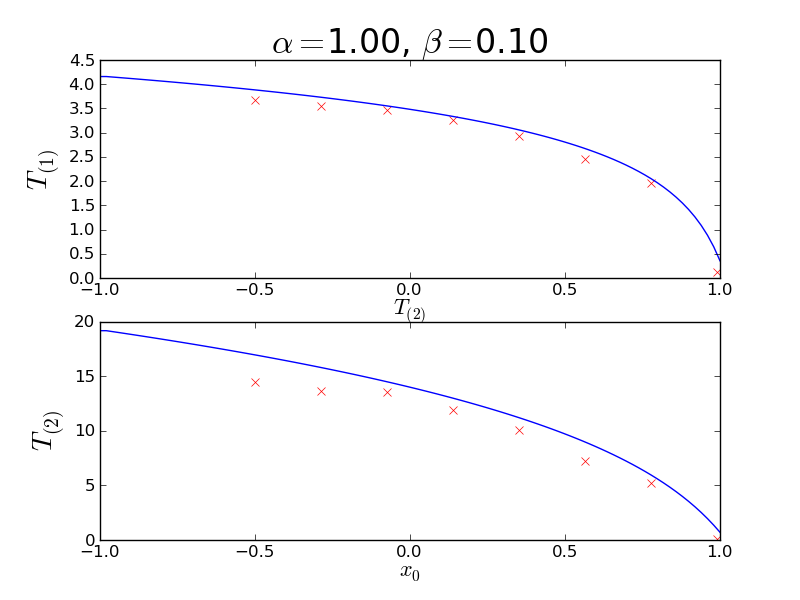
\includegraphics[width=0.48\textwidth]
{/home/alex/Workspaces/Latex/OptSpike/Figs/Moments_a=10_b=1_N=128.png}
}
\subfloat[ ]
{
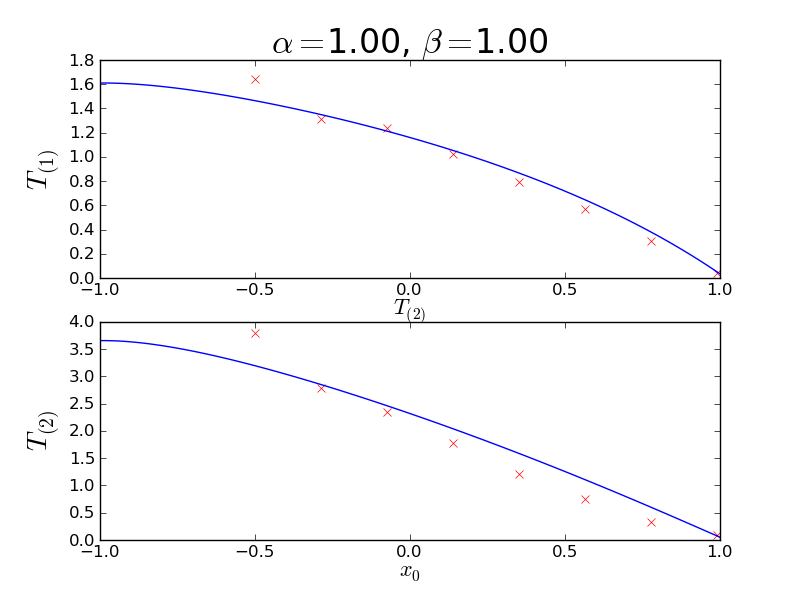
\includegraphics[width=0.48\textwidth]
{/home/alex/Workspaces/Latex/OptSpike/Figs/Moments_a=10_b=10_N=128.png}
}
\\
\subfloat[ ]
{
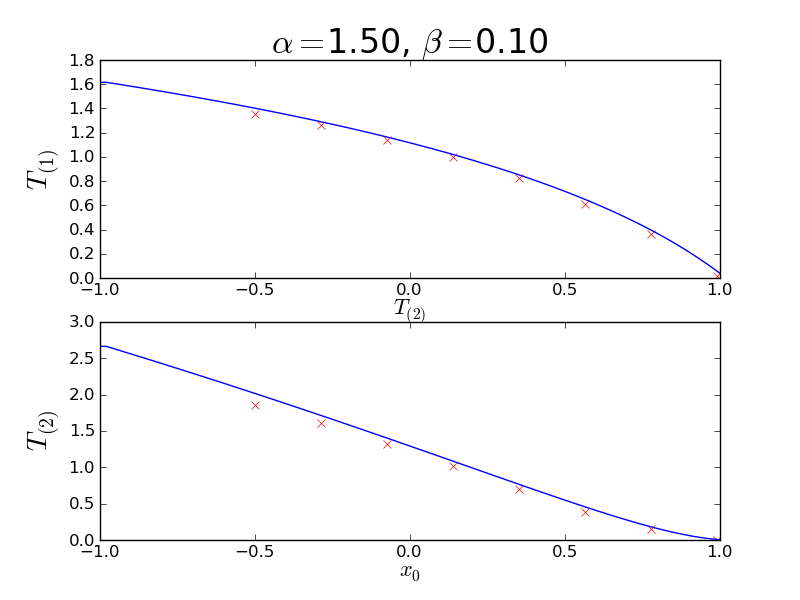
\includegraphics[width=0.48\textwidth]
{/home/alex/Workspaces/Latex/OptSpike/Figs/Moments_a=15_b=1_N=128.png}
}
\subfloat[ ]
{
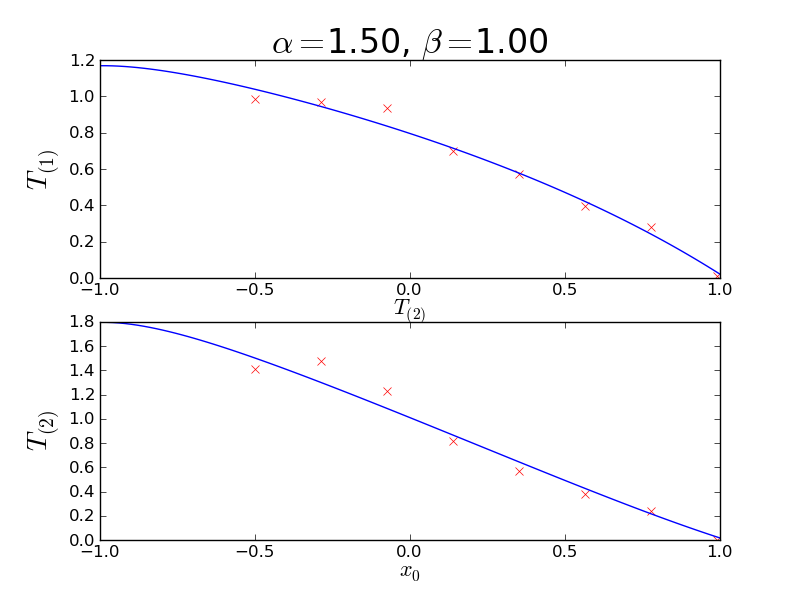
\includegraphics[width=0.48\textwidth]
{/home/alex/Workspaces/Latex/OptSpike/Figs/Moments_a=15_b=10_N=128.png}
}
\caption[]{Comparison between solutions of equations
\cref{eq:BVP_Tone,eq:BVP_Ttwo} and empirical statistics from simulating the
hitting times of \cref{eq:X_evolution_uo} for four different pairs of $\a,\b$.
In the top panel we show the first moment of the remaining time-to-spike
starting from $x$, $\Tone(x)$, and in the bottom panel, we show the second
moment, $\Ttwo(x)$. We have used only $N=128$ samples to form the moment
statistics.}
\label{fig:Ti_empirical_vs_analytic}
\end{center}
\end{figure}


\subsection{Solving the HJB - the numerical method for
\cref{eq:OC_LS_mean_HJB_bounded_control}}
We now have a PDE for $v$ and an algorithm for computing all the BCs and TCs of
this PDE. It is time to discuss the numerical method for solving
\cref{eq:OC_LS_HJB_full}.
Since we are in 1-d and we have the simplest geometry, the simplest thing to do
is try a centred Finite Difference scheme, upwind wherever necessary and hope
for the best. 

Things will break down if $\e$ is very small in which case the quadratic term,
$(\di_x v)^2 / \e$, will dominate and cause 'havoc' or if $\b$ is very small in
which case the smoothing effect of the second derivative will be negligible and
we will be in the zone of nonlinear conservation equations. Let us hope for the
best now and assume these two problems do not arise, for the parameters we
select.

Recall that we are solving backwards in time. Then for variables at the next
time-step (already computed) we will write $(\cdot)^+$; while variables at the
previous time step (to-be computed), will be denoted as$(\cdot)^-$.

Similarly given some node in space, we will write
$(\cdot)_-,(\cdot)_0,(\cdot)_+$ as the left node, the node itself and the right
node.

Then our finite-difference scheme in time looks like:
\begin{equation}
\frac{v^- - v^+}{\Delta t} = \tfrac{\b^2}2  .5*(\di_x^2 v^- + \di_x^2 v^+) +
(\a^+ - \tfrac{x}{\tc})  .5*(\di_x v^- + \di_x v^+) + \e (\a ^+)^2
\end{equation}

I.e.\ we have removed the non-linearity in $v$ by computing the control, $\a$ at
the next, already computed, time-step and used central-differencing
otherwise. 

For the spatial derivatives, we will not upwind for now and also use central
differencing:
$$\di_x v = \frac{v_+ - v_-}{2\Delta x}$$
and as is standard:
$$\di^2_x v = \frac{v_+ - 2 v_0 + v_-}{(\Delta x)^2}$$

We will not discuss a detailed study of the convergence properties of the
numerical method, but just demonstrate its performance on a representative
parameter set in \cref{fig:HJB_attempt} we see that the method is stable for a
particular parameter set. 

% \begin{figure}[ht]
% \begin{center}
%   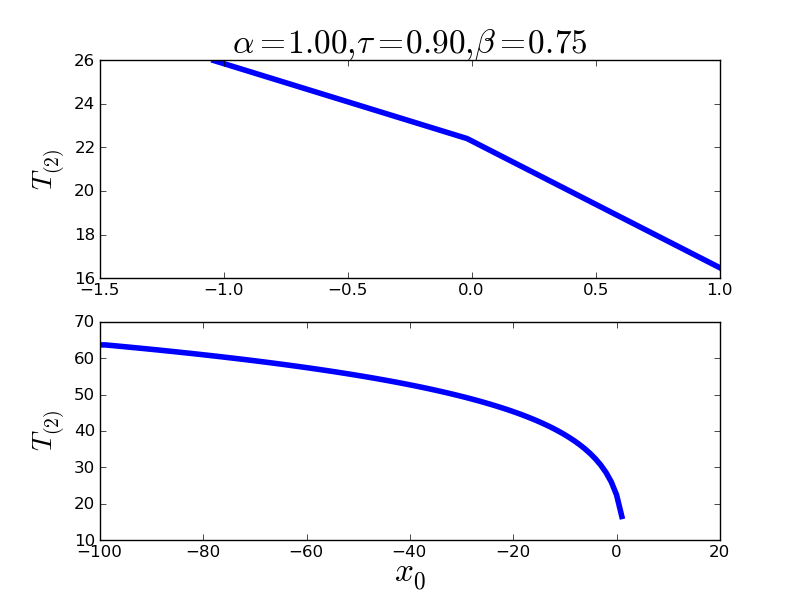
\includegraphics[width=.7\textwidth]{Figs/KolmogorovBVPMoments_a=10_t=9_b=8.png}
%   \caption[]{TCs for alpha = 1.0;  tauchar = .9; beta = .75;}
%   \label{fig:TCs_extended_x}
% \end{center}
% \end{figure}

Let's discuss the most salient features of \cref{fig:HJB_attempt}. At the end,
when $t = \T$, the value function, $v$ is monotonely decreasing. This makes
sense, becaue the lower $x$ is the more time on average will it take us to spike
and the more delay will we have from our desired spike time. However, as we go
back in time $v$ inverts, in the sense that for $t \ll \T$, we would like to
be somewhat far from the boundary to avoid the risk of spiking early.

Now focus on the controls, \cref{fig:HJB_attempt_control}: Naturally, at the
end we have the control assume its maximum value, $\a(t>=\T) = \amax$. As we
start to go back in time however, two things start to happen, the control $\a$
decreases for $x \ll \xth$, and it becomes negative for $x \lesssim \xth$. 
That is fully consistent with the problem objective - for
$t<\T$, we want to distance $X_t$ from the threshold to avoid an early spike.
\begin{figure}[h!]
\begin{center}
\subfloat[Solution, $v$]
{
\label{fig:HJB_attempt_soln}
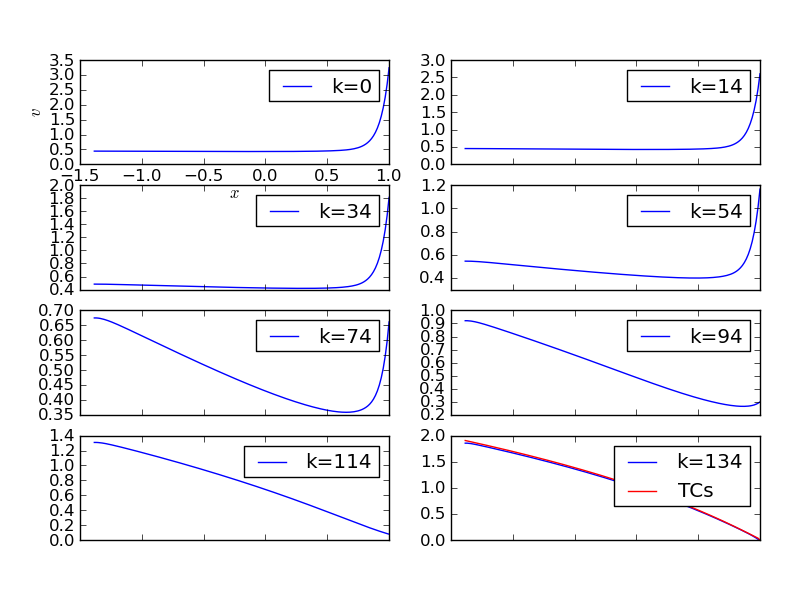
\includegraphics[width=0.48\textwidth]
{Figs/HJB/soln_al=-20_au=20__t=5_b=8.png}
}
\subfloat[Controls, $\a$]
{
\label{fig:HJB_attempt_control}
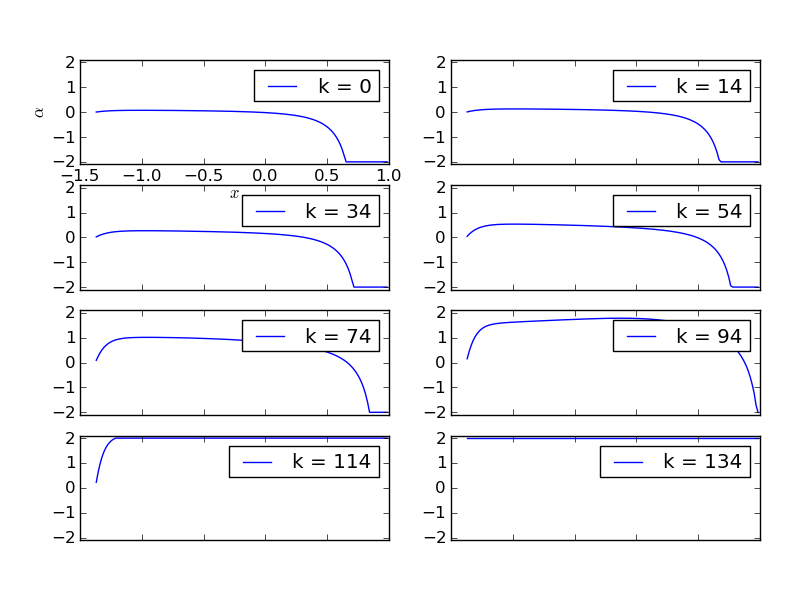
\includegraphics[width=0.48\textwidth]
{Figs/HJB/control_al=-20_au=20__t=5_b=8.png}
}
\caption[]{The solution and controls for the HJB PDE parametrized by:
$\tc = 0.50,  \beta = 0.75,
\amin = -2.00, \amax = 2.00, \eps=0.10,
\T = 1.80$. The $k$ index indicates the time-step, and recall that we are
running backwards in time, so the computation actually happens from right-to-left, bottom-to-top}
\label{fig:HJB_attempt}
\end{center}
\end{figure}

\section{Deterministic Control}
\label{sec:deterministic_ode_control}
Now we will compute the optimal control in the case that $\b = 0$. The reason we
do this is that since we have assumed that we have no feedback, we attempt to
devise an open-controller by controlling the non-random dynamics. The
calculation of this control turns out to be very simple:

First let us assume that we actually can get to $\xth$ from $0$ in $\T$ time
given $\amax$ and no noise. 

Then 
\begin{equation}
\begin{gathered}
J = \int_0^\T \e \a^2 \intd{t}
\\
\st
\begin{cases}
\dot{x} = (\a(t) - \frac{x}{\tc})
\\
x_\T = \xth
\\
x_0 = .0
\end{cases} 
\end{gathered}
\end{equation}
The (Pontryagin) Hamiltonian becomes:
\begin{equation}
\H(x,p, \a) = \e \a^2 + p \cdot (\a - x/\tc )
\end{equation}
the adjoint is given by:
\begin{equation}
-\dot{p} = \di_x \H = - p / \tc 
\end{equation} 
and the (unconstrained) control by:
\begin{equation}
\a(t) = \frac p {2 \e}
\end{equation}
which looks very similar to the stochastic case, once you put $p = \di_x v$. 

We can actually solve for the adjoint analytically: 
$$
p = p_0 \exp(t / \tc)
$$
where we can freely choose $p_0$ to later recover the TCs for $x$.
$$
\a(t) = \frac{p_0 \exp(t / \tc)}{2\e}
$$
Finally the solution for $x$ is:
\begin{align*}
\dot{x} & = \a(t) -  \frac{x}{\tc}
\\ & = \frac{p_0 \exp(t / \tc)}{2\e} - \frac{x}{\tc}
\\
e^{t/\tc}x &= \int^t e^{s/\tc}\frac{p_0 \exp(s / \tc)}{2\e} \intd{s}
\\
x &= e^{-t/\tc} \cdot \frac{p_0 }{2\e} \tc \left[  \exp(2 t / \tc) -1 \right] 
\\
&= \frac{p_0 }{\e} \tc \cdot  \sinh (t/ \tc)
\end{align*}
And so: 
$$
x(\T) = \xth \implies p_0 = \e \frac{\xth  }{ \tc \sinh (\T/ \tc) }
$$
And we have a full solution.

If we have saturation, i.e. if $\a$ hits its upper bound, then the situation is
mildly more complicated. Since $p$ is monotonically increasing, as long as $p_0
> \amin$ then $\a(t) > \amin \forall t$. So the saturation is simplified to:
\begin{equation}
\a(t) = \min \left(\frac{p_0 \exp(t / \tc)}{2\e} , \amax \right)
\label{eq:deterministic_control_bounds}
\end{equation}
In particular, $\a$ will start by following $p(t)$ and then eventually hit its
upper bound and stay there until $\T$. 

The only complication then is to calculate when $\frac{p_0 \exp(t / \tc)}{2\e} =
\amax$ and then redo the calculation for $x$ with the new control in order to
obtain the new value of $p_0$. Or we can just brute-force solve for $p_0$, by a
simple shooting method. Using the latter approach, a solution-control pair for
the parameter set we will use later is shown in \cref{fig:deterministic_soln_controls}. 
%\usepackage{graphics} is needed for \includegraphics
\begin{figure}[htp]
\begin{center}
  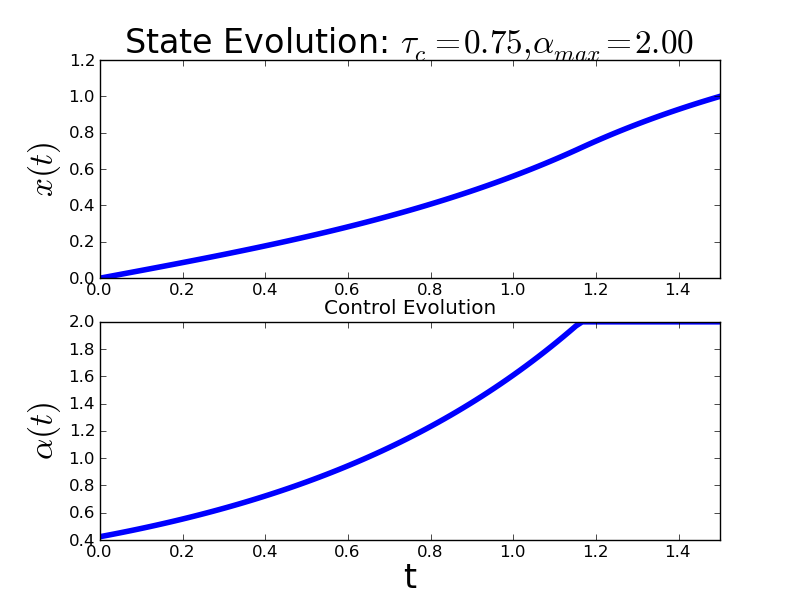
\includegraphics[width=.7\textwidth]{Figs/ControlSimulator/deterministic_example.png}
  \caption[]{An example trajectory for the deterministic dynamics. Above is the
  state evolution, $x(t)$ given $\b=0$ and below is the applied control,
  $\a(t)$. }
  \label{fig:deterministic_soln_controls}
\end{center}
\end{figure}

\section{Open-loop Stochastic Control}
As we have mentioned before, when the value of $X_t$ is unknown, the best one
can do is to use the transition density to perform the optimization. Since the
transition density follows a (deterministic) PDE, we will thus apply a Maximum
Principle for PDEs as a method of obtaining the optimal control. 

\subsection{Fokker-Planck equation for the state density evolution}

We will need the transition density of $X$, conditional on no
spikes having occurred. We will write this as:
\begin{align*}
f(x,t) \intd{x} &= \Prob[X_t\in \intd{x} | X_0 = .0, X_{s<t} < \xth]  								  
\end{align*}
Then $f$ satisfies a Fokker-Planck equation with absorbing boundaries
\begin{equation}
\begin{gathered}
\di_t f(x,t) =
				\frac{\b^2 }{2}\cdot \di^2_x f -  
				\di_x \Big[ (\a(t)- \frac{x}{\tc})  \cdot f \Big]
\\
\\
\begin{array}{lll}
	&\textrm{st.\ }& 
	\left\{ \begin{array}{lcl}
	 f(x,0) &=& \delta(x) \quad (\textrm{delta function}
	\\
	(\a(t)- \tfrac x \tc)f - \di_x \tfrac {\b^2}2 f] \big|_{x=\xmin} &\equiv& 0
	\quad (\textrm{reflecting BCs at some } \xmin )
	\\
	f(x,t) |_{x=\xth} &\equiv& 0 \quad (\textrm{absorbing BCs at } \xth)
\end{array} \right. 
\end{array}
\label{eq:FP_pde_OU_PDF}
\end{gathered}
\end{equation}
In theory, $\xmin = -\infty$, but in the numerics below we will need to
truncate it to some finite value.

The probability flow, $\phi$, here is
$$
\phi(x,t) = (\a- \tfrac x \tc)f - \di_x [\tfrac {\b^2}2 f]
$$
as such the $f$ dynamics can also be written as:
$$
\di_t f(x,t) = - \di_x \phi(x,t)
$$
and the lower BC is:
$$
\phi(x,t) |_{x=\xmin} \equiv 0
$$

We will also need a short hand notation for the differential operator on the
right side of \cref{eq:FP_pde_OU_PDF}. Let
$$
\L_\a[\cdot] := \di^2_x [ \frac{\b^2 }{2} \cdot] -  
				\di_x  [ (\a(t)- \frac{x}{\tc}) \cdot]
$$
This is a linear and bounded differential operator. . We will usually omit the
subscript $\a$, but have written it now, since the operator is parametrized by
$\a$, that is by the control.


\subsection{Restating the objective in terms of $f$}
Let us recall our objective, \cref{eq:OC_LS_variance}:
$$
J(\a) = \Exp\left[
(\ts - \T \big)^2 
+  
\e \int_0^\ts  \a^2(s) \intd{s}
\right]
$$
Rewriting this in terms of $f$ reads:
\begin{multline}
J(\a) = 
\int_\xmin^\xth \Ttwo(x) f(x,\T) \intd{x}
\\
+ \int_0^\ts \phi(\xth, s) (s-\T)^2 \intd{s}
\\
+  \e \int_0^\ts  \a^2(s)  \int_\xmin^\xth f(x,s) \intd{x} \intd{s}
\label{eq:OC_LS_variance_density}
\end{multline}

Let us explain in more detail each term on the RHS in
\cref{eq:OC_LS_variance_density}:

The first term
$$
\int_\xmin^\xth \Ttwo(x) f(x,\T) \intd{x}
$$
counts the cost of trajectories which spike too late:
this cost is the expected squared time-to-hit starting at $x$, with  $\a
= \amax$, weighted by the probability of $X_\T = x$ , $f(x,\T)$. Recall
that we calculated $\Ttwo(x)$ in \cref{sec:calculating_TCs}.

The second term
$$
\int_0^\ts \phi(s,t) (s-\T)^2 \intd{s}
$$
counts the cost of trajectories which spike too soon, that
is the squared difference between realized spike time, $t$ and desired spike
time $\T$, weighted by the probability of spike at $t$ which is just the outflow of
probability, $\phi(\xth,t)$. Note further that due to the homogeneous
Dirichlet BC on $f$ at $\xth$, the outflow is simply:
$$
\phi(\xth, t) = -\frac{\b^2 }{2} \di_x f(\xth, t) 
$$

Finally, the third term
$$
\e \int_0^\ts  \a^2(s)  \left[  \int_\xmin^\xth f(x,s) \intd{x} \right] \intd{s}
$$
is the energy cost: the inner integral, $\int_\xmin^\xth f(x,s) \intd{x}$
takes into account that we incur an energy cost only for those trajectories
which have not yet spiked.

With that our control $\a$ will naturally be found via:
$$
\a = \argmin J[\a]
$$

\subsection{Optimizing with $f$ using a Pontryagin-type Maximum Principle}
\label{sec:PDE_max_principle_for_pdf}
By now our ostensibly stochastic optimal control problem modelled by SDEs
has become a deterministic optimal control problem modelled by PDEs. Our control
$\a$ influences the evolution density $f$ and via $f$, the integrals in the
objective, $J$.

As in the ODE theory, we will introduce an adjoint function, $p$, which will be
crucial in setting up necessary conditions for the optimal control.

The basic formulation for the adjoint PDEs and the abstract Hamiltonian can be
found in \cite{Fattorini1999,Palmer2011}. However our cost functional is a
little strange as it involves values of $\di_x f$ at the boundary. As such we
will derive the optimality condition heuristically, appealing to the
references for rigorous proofs.

Before proceeding, one might wish to read
\cref{sec:Pontryagin_heuristic_derivation} for a simpler version of the
following derivation with exactly the same ideas.

We start by assuming that $f,\a$ are the optimum trajectory/control pair and we
ask what necessary conditions must be true for $f,\a$. In particular if we take
a small variation around $\a$, we will have:
\begin{align*}
\a_\e = \a + \e \da
\\
f_\e = f + \e \df
\end{align*}

With that the variation of the cost with respect to the control at the optimal
$\a$ can be calculated as:
\begin{equation}
\frac {dJ}{d\e} \Big|_{\e = 0} =
- \int_0^\T (s-\T)^2 \frac {\b^2}{2} \di_x  \df \intd{s}  
+ \int_\xmin^\xth \Ttwo\df\intd{x}
+ \tilde{\e} \int 2 \a \da \intd{s}  
\label{eq:J_variation_PDE}
\end{equation}
This must be non-negative for a true minimum, but before we can say more, we
need to eliminate $\df$ from $\frac {dJ}{d\e}$! In order to eliminate $\df$
from \cref{eq:J_variation_PDE} we will introduce an adjoint variable, $p$. What
we would want from this adjoint variable $p$ would be that:
\begin{equation}
p(x,\T) = \Ttwo(x)
\label{eq:adjoint_TC_desideratum}
\end{equation}  
and 
\begin{equation}
\di_t \left[ \int_\xmin^\xth  p \cdot\df \intd{x} \right] = (s-\T)^2 \frac
{\b^2}{2}
\di_x
\df
 + \text{stuff}
\label{eq:adjoint_dynamics_desideratum}
\end{equation}
where 'stuff' does not depend on $\df$.

If we had such a $p$ satisfying
\cref{eq:adjoint_TC_desideratum,eq:adjoint_dynamics_desideratum} then
\cref{eq:J_variation_PDE} would read:
\begin{equation}
\frac {dJ}{d\e} \Big|_{\e = 0} =
\tilde{\e} \int 2 \a\da  \intd{s} +   \int_0^\T  \text{'stuff'}\intd{s}
\label{eq:J_variation_PDE_nodf}
\end{equation}
which does not depend on $\df$! and we would be on our way. In order to find
$p(x,t)$ we will need to
\begin{enumerate}
  \item calculate $\di_t \df$
  \item specify $\di_t p $ st. \cref{eq:adjoint_dynamics_desideratum} holds.
\end{enumerate}

\subsection{The PDE for $\df$}
First, calculate the PDE that $\df$ satisfies:
\begin{multline}
\di_t f_\e =  \L_{\a_\e} [f_\e]
\\
= -\di_x [ (\a_\e - \tfrac{x}\tc) f_\e  - D \di_x f_\e]
\\
=  -\di_x [ (\a + \e\da - \tfrac{x}\tc) f_\e  - D \di_x f_\e]
\\
=  -\di_x [ (\a + \e\da - \tfrac{x}\tc) (f + \e \df)  - D \di_x (f + \e \df)]
\\
=  -\di_x [ (\a + \e\da - \tfrac{x}\tc) (f)  - D \di_x (f)]
- \di_x [ (\a + \e\da - \tfrac{x}\tc) (\e \df)  - D \di_x (\e \df)]
\\
= \L_\a f  -\di_x [ \e\da\cdot  f]
  +\e \L_\a \df + o(\e) 
\\
= \di_t f + \e \di_t \df
\end{multline}
Of course, we have $\di_t f = \L_\a f$, so we conclude that:
\begin{equation}
\di_t \df = \L_\a \df -\di_x [\da \cdot f] 
\end{equation}
Now what are the ICs? Well, both $f_\e$ and $f$ must satisfy the system ICs in
\cref{eq:FP_pde_OU_PDF}, so $$\df (x,0) = 0$$.
Finally, what are the BCs?
On the upper side:
$$
f_\e |_\xth = 0 = [ f  + \e \df |_\xth = 0 + \e \df|_\xth \implies \df |_\xth =
0 $$
While on the lower side:
\begin{align*}
0 =& [ (\a_\e - x/\tc)f_\e - D \di_x f_\e |_\xmin
\\
=& (\a +\e \da - x/\tc)(f + \e \df ) - D \di_x (f + \e \df) |_\xmin
\\
=& [(\a +\e \da - x/\tc)(f) - D \di_x (f) |_\xmin
\\
& + \e [ (\a +\e \da - x/\tc)(\df) - D \di_x (\df) |_\xmin
\\
=& \cancel{[(\a - x/\tc)f - D \di_x (f) |_\xmin}
\\
&+ \e \da f|_\xmin
\\
&+ \e [ (\a - x/\tc)(\df) - D \di_x (\df) |_\xmin   + o(\e)
\end{align*}
 
so $\df$ satisfies the following system of equations:
\begin{equation}
\begin{gathered}
\begin{aligned}
\di_t \df 
&= \L_\a \df -\di_x [\da \cdot f]
\\
&= -\di_x \left[ (\a - \tfrac x\tc)\df - \tfrac{\b^2}2 \di_x \df \right]
-\di_xf \cdot\da
\end{aligned}
\\
\begin{cases}
\df(x,0) &= 0
\\
[ (\a - \frac x \tc)(\df) - D \di_x (\df) |_\xmin &= -\da \cdot f|_\xmin
\\
\df|_\xth &= 0
\end{cases}
\end{gathered}
\label{eq:FP_variation_near_optimum}
\end{equation} 
With \cref{eq:FP_variation_near_optimum} we are ready to design the dynamics of
$p$ such that $\df$ is eliminated from the optimality equation,
\cref{eq:J_variation_PDE}.

\subsection{Calculating the adjoint }
Recall our desideratum, we want
$$
p(x,\T) = \Ttwo(x) \quad (\text{required TCs})
$$
and
$$
\int_0^\T \di_t (p \cdot \df) = \int_0^\T(s-\T)^2 \frac {\b^2}{2} \di_x 
\df \intd{s} + \text{stuff}
$$
This is equivalent to having
$$
\di_t (p \cdot \df) =  (s-\T)^2 \frac {\b^2}{2} \di_x 
\df  + \text{stuff}
$$
Let us calculate $\di_t (p \cdot \df)$
\begin{align*}
\di_t (p \cdot \df) =& \df \cdot \di_t p + p \cdot   \di_t \df
 \\
 =& \df \cdot \di_t p + p \cdot \left( \L [\df] -\di_xf \cdot\da \right)  
 \\
 =& \df \cdot \di_t p + p \cdot \L  [\df] - \underbrace{ p \cdot \di_xf \cdot\da}_{\text{stuff}}
\end{align*}
Now our job is clear - we want 
$$
\di_t p = -\Lstar[p]
$$
Where $\Lstar$ is defined by:
\begin{equation}
\begin{gathered}
\int_\xmin^\xth  \Lstar [p] \df \intd{x} 
=
\int_\xmin^\xth p \L [\df] \intd{x} - (s-\T)^2 \frac {\b^2}{2}\di_x \df +
\text{possibly more stuff}
\\
\\
\forall \df \quad \st \begin{cases}
\df(x,t) |_{x=\xth} & = 0 
\\
(\a - \tfrac x \tc)\df - \di_x \tfrac {\b^2}2 \df \big|_{x=\xmin} &=  -\da
\cdot f
\end{cases}
\end{gathered}
\end{equation}
where 'possibly more stuff' should be independent of $\df$.

Let us take a deep breath and calculate $\Lstar$:
\begin{align*}
\int p \L [\df] \intd{x} =&
\int p \underbrace{\left(\frac{\b^2 }{2}\cdot \di^2_x \df -  
			 \di_x \big[ (\a- \frac{x}{\tc})\cdot \df \big]\right)}_{\L [\df]} \intd{x}
\\
=& [ -p ((\a- \frac{x}{\tc})  \cdot \df)\quad  \vert^\xth_\xmin
+ \int \di_xp ((\a- \frac{x}{\tc})  \cdot \df) \intd{x}
\\
& + [p (\frac{\b^2 }{2}\cdot \di_x \df \quad \vert ^\xth_\xmin
- [ \di_x p \cdot \frac{\b^2 }{2}  \df\quad \vert^\xth_\xmin 
+ \int \frac{\b^2 }{2} \di^2_xp    \cdot \df \intd{x} 
\\
=& \int \Lstar [p] \df \intd{x} 
+\underbrace{[-p(\a- \frac x \tc) \cdot \df 
+ p \frac{\b^2}{2} \di_x \df 
-\di_x p \frac{\b^2}{2} \df \,\vert^\xth_\xmin }_{\text{BC terms}}
\end{align*}

Now we want to make the 'BC terms' equal to $(s-T)^2 \frac{\b^2}{2} \di_x \df$
+ 'possibly more stuff'.
In doing so, we will discover the correct BCs associated with the adjoint
operator, $\Lstar$:
\begin{align*}
\textrm{BC terms} =& 
\Big[ -p (\a- \frac{x}{\tc})  \cdot \df 
+ p \frac{\b^2 }{2}\cdot \di_x \df   
- \di_x p \cdot \frac{\b^2 }{2}  \df   \quad ^\xth_\xmin\vert 
\\
=& -\cancel{p (\a- \frac{x}{\tc})  \cdot \df \Big|_\xth}
 + p (\a- \frac{x}{\tc}) \cdot \df \Big|_\xmin
\\ 
& + [p \frac{\b^2 }{2}\cdot \di_x \df \Big|_\xth
 - [p \frac{\b^2 }{2}\cdot \di_x \df \Big|_\xmin
\\
&- \cancel{[ \di_x p \cdot \frac{\b^2 }{2}   \df\Big|_\xth}
 + [ \di_x p \cdot \frac{\b^2 }{2}   \df\Big|_\xmin
\\
=& \cancelto{-p (-\da f)}{-p ((\a- \tfrac x \tc)\df - \di_x \tfrac {\b^2}2
\df) \Big|_\xmin} 
+ [p \frac{\b^2 }{2}\cdot \di_x f \Big|_\xth
+ [ \di_x p \cdot \frac{\b^2 }{2}   f\Big|_\xmin
\\
=& (s-T)^2 \frac{\b^2 }{2}\cdot \di_x \df\Big|_\xth 
+  p (\da f)\Big|_\xmin
\end{align*}

Since we want this to be true for arbitrary $\df$, we need to enforce the
following (adjoint) BCs: 
$$
\begin{cases}
p |_\xth &= (s-T)^2
\\
\di_xp |_\xmin &= 0
\end{cases}
$$

In summary, the adjoint PDE equation is given by: 
\begin{equation}
\begin{gathered}
\begin{aligned}
\di_t p =& - \Lstar[p]
\\
		=&  
			- \Big[ \frac{\b^2 }{2}\cdot \di^2_x p +  
			(\a(t)- \frac{x}{\tc})  \cdot \di_x p \Big] 
\end{aligned}
\\
\st  
\begin{cases}
	p(x,\T) &= \Ttwo(x)
	\\ 
	\di_x p  \big|_{x=\xmin} &\equiv 0
	\\
	p \big|_{x=\xth} &\equiv (s-T)^2
\end{cases}
\label{eq:adjoint_pde_OU}
\end{gathered}
\end{equation} 

And most importantly:
\begin{equation}
\int \Lstar [p] \df \intd{x}
=  
\int p \L [\df] \intd{x} 
  - (s-T)^2 \frac{\b^2 }{2}\cdot \di_x \df\Big|_\xth 
  -  p  f \cdot \da \Big|_\xmin
\label{eq:L_to_Lstar_relation}
\end{equation}

\subsection{A Pontryagin-type Minimum Principle for the optimal control $\a$}
Using \cref{eq:L_to_Lstar_relation} and the TCs in \cref{eq:adjoint_pde_OU}, we
will have:
\begin{align*}
\int \Ttwo \df \intd{x} =& 
\int_\xmin^\xth p \df \intd{x}
\\ =& \int_0^\T \di_t \int_\xmin^\xth p \cdot \df \intd{x} \intd{s}
\\
=& \int_0^\T \int _\xmin^\xth - \df \cdot \Lstar[p]
 + p \cdot \L_\a [\df] 
 -  p \cdot \di_x [\da \cdot f]  \intd{x}  \intd{s}
\\
=& 
\int_0^\T \Big\{  (s-T)^2 \frac{\b^2 }{2}\cdot \di_x \df\Big|_\xth 
+  p (\da f)\Big|_\xmin
\\
& \quad
- \int _\xmin^\xth p \cdot \di_x [\da \cdot f] \intd{x} \Big\} \intd{s}
\end{align*}

Now put this back into the equation of optimality, \cref{eq:J_variation_PDE}.
\begin{align*}
\frac {dJ}{d\e} \Big|_{\e = 0} =&
- \int_0^\T (s-\T)^2 \frac {\b^2}{2} \di_x  \df \intd{s}  
+ \int_\xmin^\xth \Ttwo\df\intd{x}
+ \tilde{\e} \int 2 \a \da \intd{s}
\\
=& 
\int_0^\T \Big\{
 p (\da f)\Big|_\xmin
+ \tilde{\e}  2 \a \da
- \int _\xmin^\xth p \cdot \di_x [\da \cdot f] \intd{x} 
 \Big\} \intd{s}
 \\
=& 
\int_0^\T \da \Big\{
 p f \Big|_\xmin
+ \tilde{\e}  2 \a
- \int _\xmin^\xth p \cdot \di_x f \intd{x} 
 \Big\} \intd{s}
\end{align*}

Now we pull the famous fundamental lemma of the calculus of variations out and
conclude that
\begin{equation}
\Big\{
 \tilde{\e}  2 \a(t)
+ p f \Big|_\xmin
- \int _\xmin^\xth p \cdot \di_x f \intd{x} 
\Big\} = 0
\quad \forall t \in [0,T]
\label{eq:J_necessary_condition}
\end{equation}

Working in reverse we can recognize a Hamiltonian, $\H$ as:
$$
\H(f,p,\a) =  \int \cref{eq:J_necessary_condition} \intd{\a} 
$$

Naturally, $f,p$ must satisfy their respective
\cref{eq:FP_pde_OU_PDF,eq:adjoint_pde_OU}.

And our optimal control, $\a$,  can be found via:
\begin{equation}
\a (t) = \frac { - p(\xmin,t) f(\xmin,t)
+ \int _\xmin^\xth p(x,t) \cdot \di_x f(x,t) \intd{x} 
}{2\e}
\label{eq:optimal_alpha_4_PDF_optimization}
\end{equation}
As always, subject to the appropriate bounds, \cref{eq:bound_constraints_alpha}.

\subsection{An Iterative Numerical Solution}
We have an entangled situation: $f,p$ depend on $\a$ through
\cref{eq:adjoint_pde_OU,eq:FP_pde_OU_PDF}, while $\a$, the optimal control, is
given by \cref{eq:optimal_alpha_4_PDF_optimization} which requires  the
solution to $f,p$ . So we need some kind of iteration to find $\a$ and the corresponding $f,p$.

The key to such an iteration is that the quantity 
$$\di_\a \H =  \Big\{
 \tilde{\e}  2 \a(t)
+ p(x,t) f(x,t) \Big|_\xmin
- \int _\xmin^\xth p \cdot \di_x f(x,t) \intd{x} 
\Big\}
$$
gives us the direction of increase
and we can use it as a gradient in a descent algorithm. 
This we can also write as:
\begin{align*}
\di_\a \H =&  \Big\{
 \tilde{\e}  2 \a(t)
+ p(x,t) f(x,t) \Big|_\xmin
- [p(x,t) f(x,t) \, _\xmin^\xth\Big|
+ \int _\xmin^\xth \di_x p \cdot f(x,t) \intd{x} 
\Big\}
\\
=&
 \Big\{
 \tilde{\e}  2 \a(t)
- p(x,t) f(x,t)\Big|_\xth
+ 2p(x,t) f(x,t) \Big|_\xmin
+ \int _\xmin^\xth \di_x p \cdot f(x,t) \intd{x} 
\Big\}
\end{align*}
which has certain numerical advantages.



So the plan is: we choose an initial $\a_1(t)$ - the deterministic solution
from \cref{sec:deterministic_ode_control} is a natural choice. Then solve for $f,p$.
Then evaluate $J$ and iterate until convergence. For our convergence
criterion we will take that the incremental difference in $J$ is smaller than
some difference small tolerance. The algorithm is specified more
precisely in Algorithm \ref{alg:hamiltonian_descent_4_PDF_OC}.
\begin{algorithm}
\begin{algorithmic}
\State $J_0 = \infty $ 
\State $\a_1 = $ deterministic $\a$, the optimal control given $\b=0$ from
\cref{sec:deterministic_ode_control}
\For { $k= 1\dots k_{\max}$}
	\State $\di_t f_{k} = \L_{a_{k}} [ f_{k}]$
	\State $-\di_t p_{k} = \Lstar_{a_{k}} [ p_{k}]$
	\State $J_{k} \gets J[\a_k, f_k]$
	\If {$|J_{k} - J_{k-1}| < tol $}
		\State BREAK
	\EndIf
	\State $\da = \di_a \H(f_{k} ,p_{k},  \a_{k})$

	\If {$\sup_t |\da(t)| < tol$}
		\State BREAK
	\EndIf

	\State $\a_{k+1} \gets \a_{k} - s \cdot \da  $
\EndFor
\State \Return $J_k, \a_k$
\end{algorithmic}
\caption{Optimal Control Descent Algorithm}
\label{alg:hamiltonian_descent_4_PDF_OC}
\end{algorithm}

We show one realization of $\di_a \H$ in \cref{fig:grad_aH_deterministic_alpha}.
\begin{figure}[htp]
\begin{center}
\subfloat[$\a_0$]
{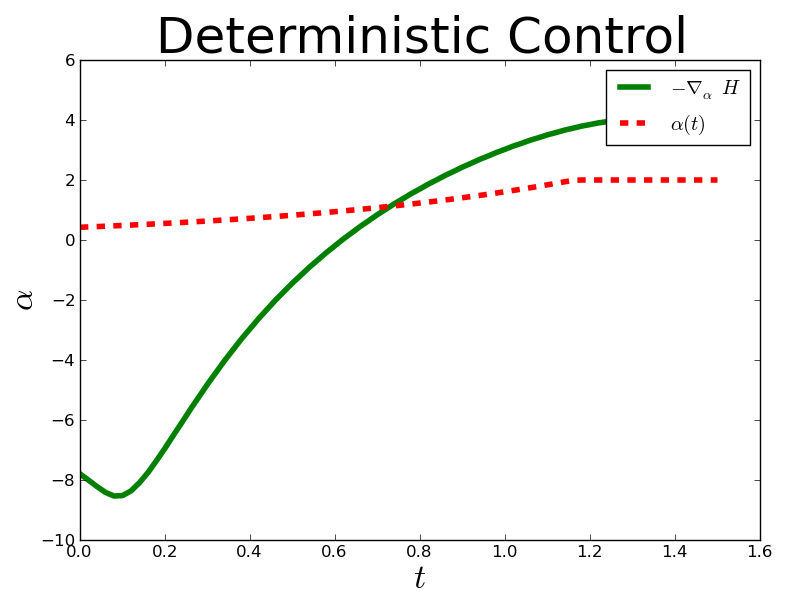
\includegraphics[width=.49\textwidth]{Figs/FP_Adjoint/Deterministic_alpha_di_aH.png}
 }
  \subfloat[$\a_1$]
{  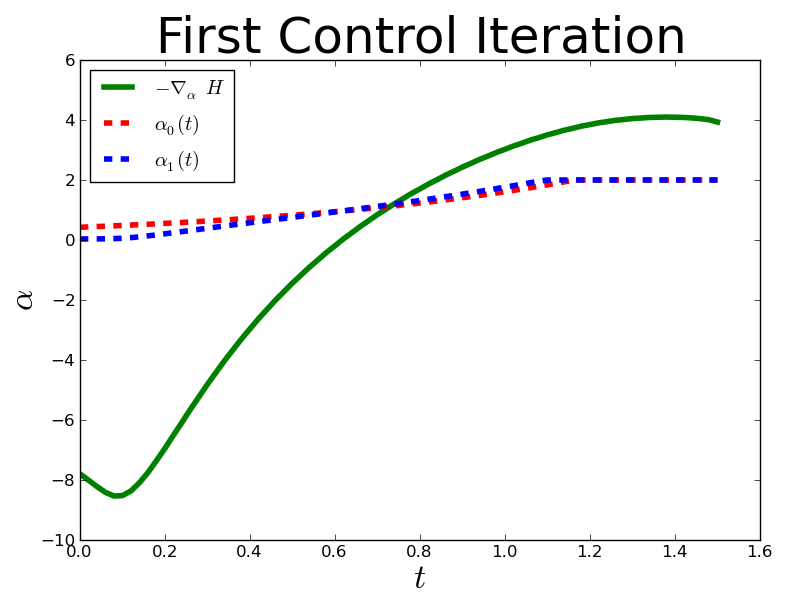
\includegraphics[width=.49\textwidth]{Figs/FP_Adjoint/First_control_iteration.png}
}
\caption[labelInTOC]{Iteratively calculating $\a$ for the
open-loop optimal control. Plotted is an example of
$-\di_a \H$ calculated at $\a(t) = \a_1(t)$, where $a_1$ is the deterministic control. The green curve, $-\di_a \H$
indicates the direction that we want to change the control, if it is negative
we decrease and if it is positive we increase it. On the right panel, b), we
show the result of applying the incremental change by also plotting the
resulting $\a_1(t)$. }
\label{fig:grad_aH_deterministic_alpha}
\end{center}
\end{figure} 

Finally, we are ready to calculate the open-loop stochastic optimal control for
this parameter set. The results are in
\cref{fig:FP_adjoint_objective_control_convergence}.

\begin{figure}[h]
\begin{center}
\subfloat[$\a_k(t)$ ]
{
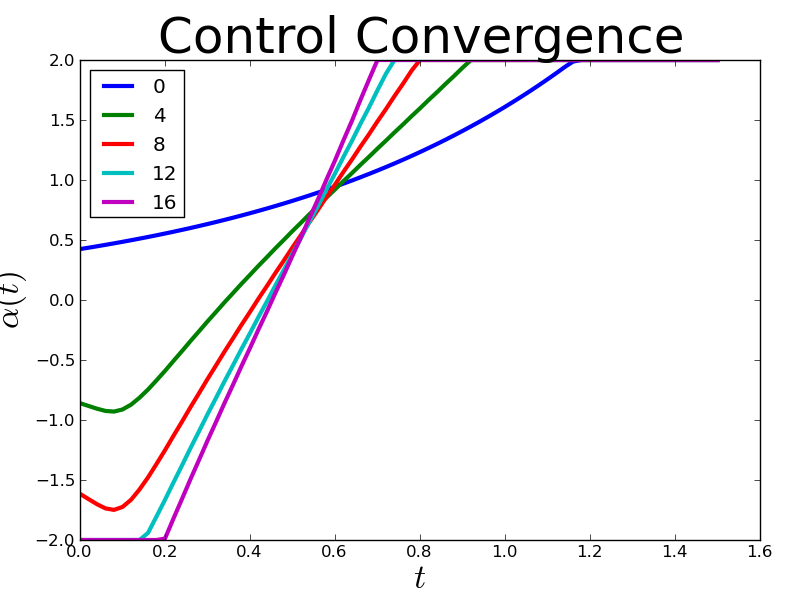
\includegraphics[width=0.48\textwidth]
{Figs/FP_Adjoint/ExampleControlConvergence_control.png}
}
\subfloat[$J_k$ ]
{
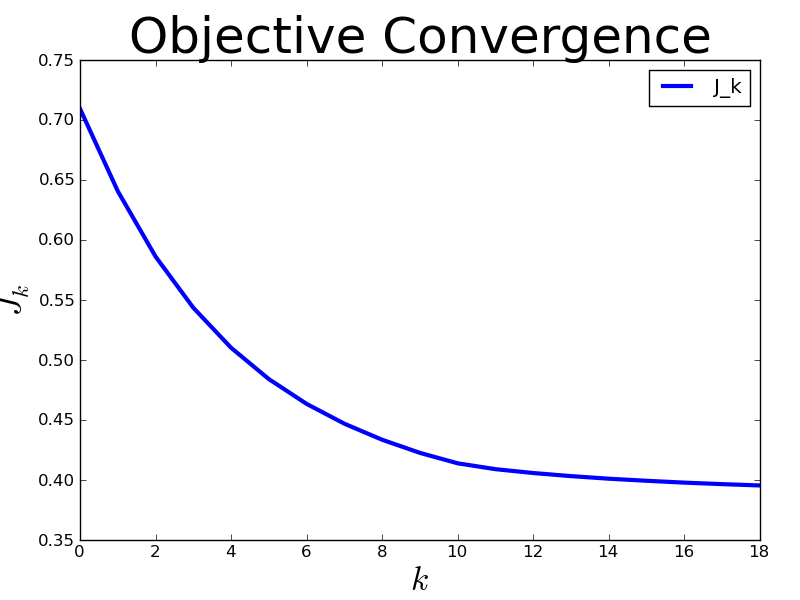
\includegraphics[width=0.48\textwidth]
{Figs/FP_Adjoint/ExampleControlConvergence_objective.png}
}
\caption[ ]{The result of an entire optimization iteration, on the left the
iterates of the control, $\a_k(t)$, on the right the progress of the
objective with each iteration. The final control, in purple, is inhibitory at
the beginning of the time interval, $\a < 0$, unlike the the deterministic
control solution. 
We see a significant
reduction in the objective value, $J$, and thus an improvement, on the
order of 50\%.}
\label{fig:FP_adjoint_objective_control_convergence}
\end{center}
\end{figure}

% \begin{table}[h] 
% \centering
% \begin{tabular}{lc}
% Control Law & Squared Error \\
% \hline
% Deterministic &  0.647 \\
% Stochastic &  0.336\\
% Theory (Value function) & 0.285
% \end{tabular}
% \caption{Realized performance of the different control laws and the theoretical
% expected performance of the stochastic law (last row)}
% \label{tab:realized_avg_errors_det_vs_stoch}
% \end{table}
% 
% \begin{figure}[h]
% \begin{center}
% \subfloat[A]
% {
% \label{fig:controlled_traj_ex1}
% \includegraphics[width=0.33\textwidth]
% {Figs/ControlSimulator/example_controlled_trajectories_id1.png}
% }
% \subfloat[B]
% {
% \label{fig:controlled_traj_ex2}
% \includegraphics[width=0.33\textwidth]
% {Figs/ControlSimulator/example_controlled_trajectories_id4.png}
% }
% \subfloat[C]
% {
% \label{fig:controlled_traj_ex3}
% \includegraphics[width=0.33\textwidth]
% {Figs/ControlSimulator/example_controlled_trajectories_id3.png}
% }
% \caption[]{Examples for the controlled trajectories using both the deterministic
% and the stochastic control approaches. The red vertical line in the plots
% indicates the desired spike-time, $\T$. In A, B the performance of both
% control laws is essentially the same, but in C we see the advantage of the
% stochastic approach. $\tc, \b = [.75, 1.25]$.}
% \label{fig:control_trajectories_examples}
% \end{center}
% \end{figure}
% \begin{figure}[htp]
% \begin{center}
%   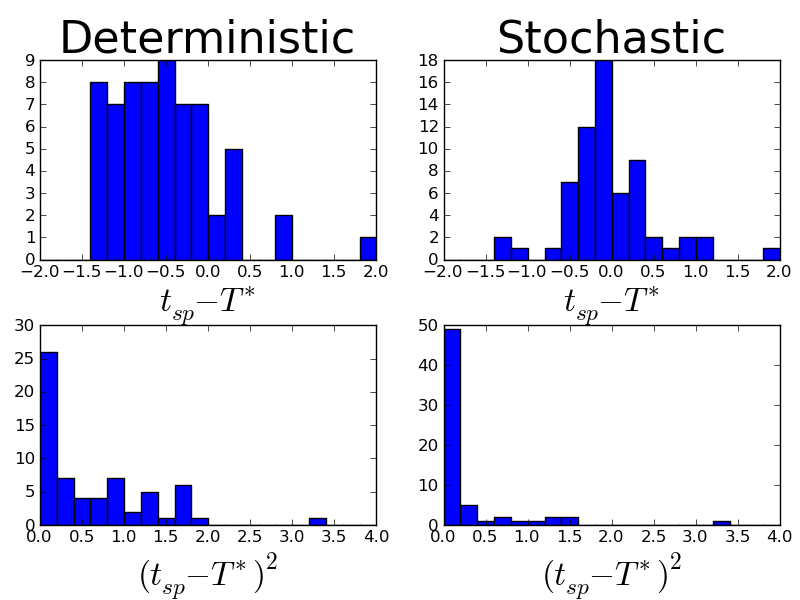
\includegraphics[width=.9\textwidth]{Figs/ControlSimulator/example_controlled_trajectories_hists.png}
%   \caption[labelInTOC]{Histogram of the spike timing error for the
%   deterministic (left) vs. the stochastic (right) control laws.}
%   \label{fig:error_histograms_det_vs_stoch}
% \end{center}
% \end{figure}


\section{Test Comparison of Different Controls}
\label{sec:probabilistic_numerical_test}
We will now compare the performance of the three obtained controls: the
closed-loop stochastic obtained via the HJB equation, the open-loop
deterministic control obtained when setting $\b=0$ and the open-loop stochastic
control obtained by optimizing using the transition density.

For our comparison we will sample $128$ realizations of the controlled system
and apply in turn each of the three controls. Naturally, for each path, we will
apply exactly the same random disturbances to each controller.

We will set $\e = .001$ and $\amax = 2.0$. As such the energy cost is of
secondary importance and the paramount effect on the objective is the difference
$(\ts - \T)$, which we are trying to minimize. We set $\tc, \b = [.75, 1.25]$.

The performance of the three controllers is given in
\cref{tab:realized_avg_errors_det_vs_openloop_vs_stoch}. We see that while the
open-loop stochastic control is not as good as the feedback stochastic
control, it is much closer in performance to it than to the blind
deterministic control.

For illustration sake, we also show the error
histograms in \cref{fig:error_histograms_det_vs_openloop_vs_stoch} and visualize
some trajectories in \cref{fig:control_trajectories_examples}.

\begin{table}[h] 
\centering
\begin{tabular}{lcc}
Control Law & Empirical Squared Error & Theoretical Squared Error \\
\hline
Deterministic &  0.621 & - \\
Open-Loop Stochastic & 0.356 & 0.382\\
Feedback Stochastic &  0.288& 0.285\\
\hline
\end{tabular}
\caption{Realized and theoretical performance of the different control laws. The empirical
performance is obtained using 128 sample paths. The theoretical performance is
found using the $J$ in for the open-loop stochastic control and the value
function $v(x=0, t =0)$ for the closed-loop stochastic control.}
\label{tab:realized_avg_errors_det_vs_openloop_vs_stoch}
\end{table}
\begin{figure}[h]
\begin{center}
\subfloat[]
{
\label{fig:controlled_traj_ex1}
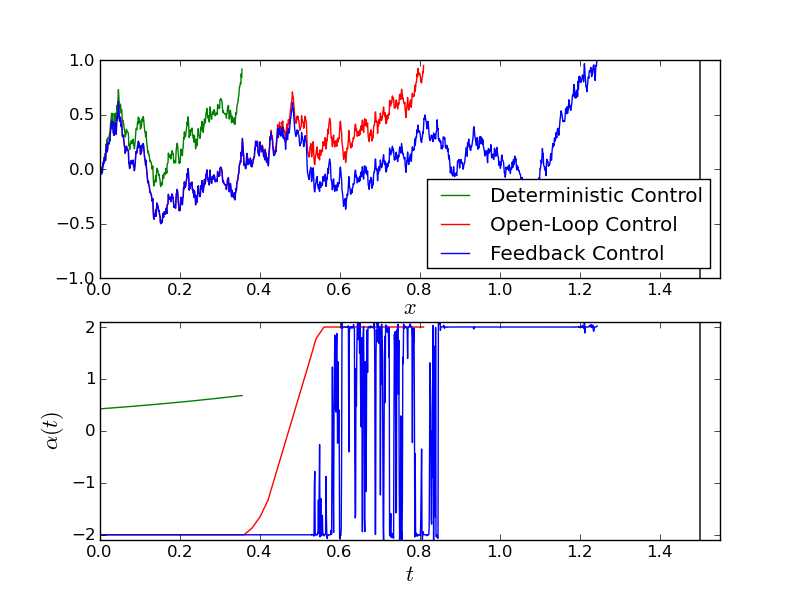
\includegraphics[width=0.33\textwidth]
{Figs/ControlSimulator/3controls_example_trajectories_id3.png}
}
\subfloat[ ]
{
\label{fig:controlled_traj_ex2}
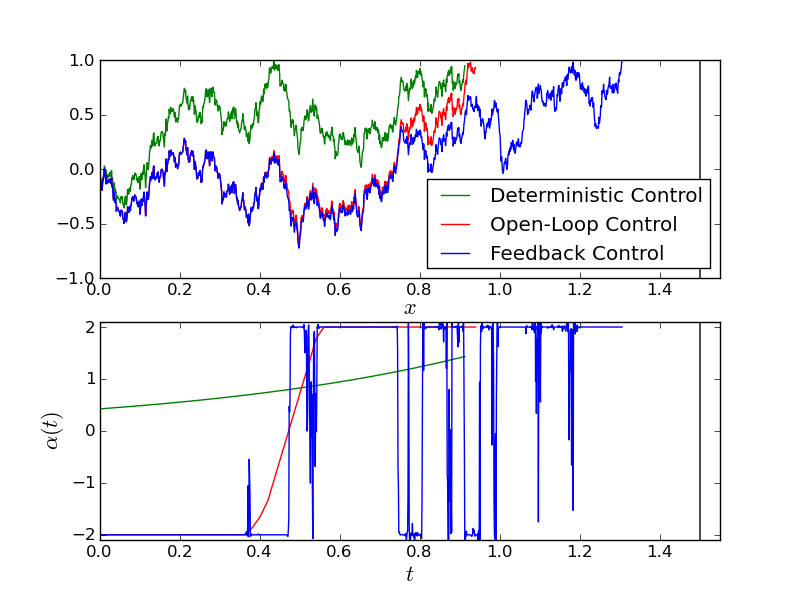
\includegraphics[width=0.33\textwidth]
{Figs/ControlSimulator/3controls_example_trajectories_id5.png}
}
\subfloat[ ]
{
\label{fig:controlled_traj_ex3}
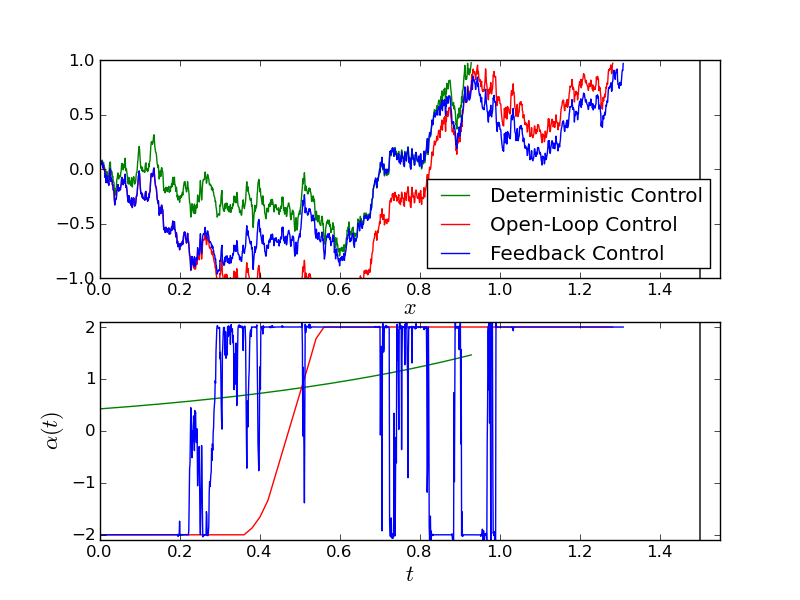
\includegraphics[width=0.33\textwidth]
{Figs/ControlSimulator/3controls_example_trajectories_id6.png}
}
\caption[]{Examples for the controlled trajectories using the deterministic,
open-loop stochastic and feedback stochastic control approaches. The
black vertical line in the plots indicates the desired spike-time, $\T$.
For the parameter values are $\tc, \b = [.75, 1.25]$. The three panels are
three different realizations of the model dynamics.}
\label{fig:control_trajectories_examples}
\end{center}
\end{figure}

\begin{figure}[h]
\begin{center}
  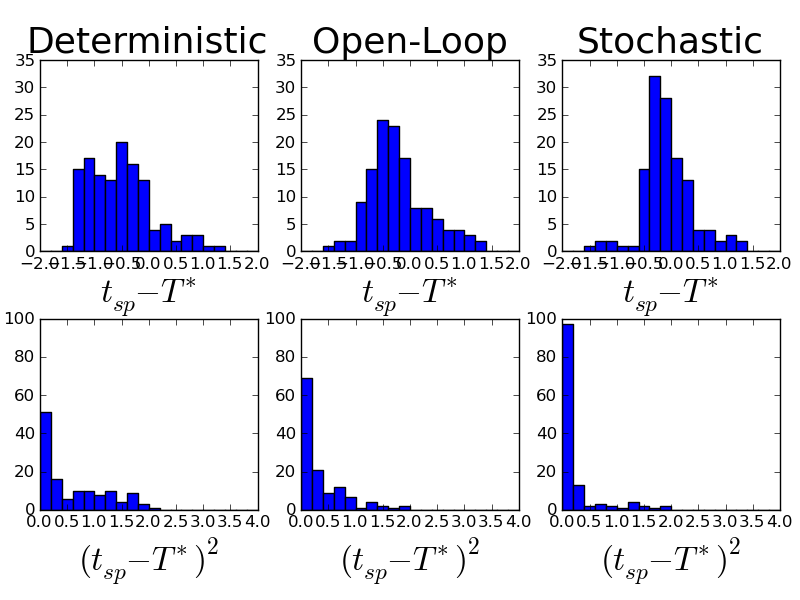
\includegraphics[width=.95\textwidth]
  {Figs/ControlSimulator/3controls_example_trajectories_hists.png}
  \caption[labelInTOC]{Histogram of the spike timing error for the
  deterministic (left) vs. open-loop stochastic(centre) vs. feedback stochastic
  (right) control laws. This is for the same problem as in
  \cref{fig:control_trajectories_examples}. We have used $N=128$ sample paths
  to form the statistics}
  \label{fig:error_histograms_det_vs_openloop_vs_stoch} 
\end{center}
\end{figure}


\section{Research Goals}
I hope to be able to use the techniques of open-loop stochastic control
discussed herein to address problems in stochastic control where for whatever
reasons, the dynamic programing formalism is not applicable. 

One such reason might be that the state is unobservable. An example of such a
system is the control of blood glucose for diabetes or intensive care
patients, where the patients' blood glucose is modelled to follow a stochastic
differential equation and actual observations are expensive and invasive and
thus rare, on the order of a few hours. In this scenario, the applied external
glucose or insulin to the patient in the time in-between measurements can be
thought of as the solution to an optimal control problem where the objective is
to minimize deviations of the patient's blood glucose from some baseline. 

An alternative reason to use the open-loop control techniques is when optimizing
with multi-dimensional systems at which point the dynamic programing approach
suffers from 'the curse of dimensionality' which is the colloquial name for the
exponential increase in necessary computing resources. If the optimality
conditions for the open-loop control lend themselves to a Feynman-Kac-type
representation, then one might replace solving the PDEs by an appropriate
Monte-Carlo process and thus make the computations tractable.
 
\clearpage
\appendix
\section{Heuristic Derivation of Pontryagin's Minimum Principle}
\label{sec:Pontryagin_heuristic_derivation}
Here we will show a heuristic derivation for the Pontryagin Minimum Principle
for linear ODE dynamics. It should motivate the manipulations in
\cref{sec:PDE_max_principle_for_pdf}.

The following is almost a direct transcription of A.1 in
\cite{Evansb}, with the added simplification of linear dynamics
and linear cost and with the notation adapted to what we have used
hereto.

The dynamics are given by:
$$
\dot{x} = A(t, \a) x
$$
where $A$ is a matrix in $\R^{n_x \times n_x}$ whose values depend on the
time, $t$ and the control $\a$. The cost, $J$, is given by:
$$
J[\a] = \int_0^\tf L(t,\a) \cdot x \intd{s} + M \cdot x(\tf)
$$
where $L(t,\a), M$
are vectors in $\R^{n_x}$. Both the dynamics and the cost are linear in the state $x$.
Suppose $x,\a$ are the optimal trajectory - then small variations in $\a$ can
only worsen $J$. Let such an acceptable variation be given by:
$$
\a_\e = \a + \e \b
$$
for some small $\e$. We will have a corresponding dynamic, $x_\e$ st:
$$
x_\e = x + \e \dx+ o(\e)
$$
Now obtain a differential equation for the variation $\dx$:
\begin{align*}
\dot{x_\e} &=  \dot{x} + \e \dot{\dx} 
\\
&= A(\a_\e) x_\e = A(\a) x + \e \dot{\dx}
\end{align*}
Now divide through by $\e$ and let it go to zero:
$$
\implies \dot{\dx} = A \dx + [\grad_\a [ A(t,\a)x]] \cdot\b
$$
Note that $$\dx(0) = 0$$ since $x(0)$ is specified and so there is no
variation there.

With that the derivative of $J$ at $\a$ will read:
\begin{multline}
\frac {dJ}{d\e} \Big|_{\a} = \lim \frac{ J[\a_\e] - J[\a]}{\e} 
= \int L(\a,t) \dx +  \grad_\a L \cdot \b \intd{s} + M \dx(\tf)
\geq 0 
\label{eq:J_variation_ODE}
\end{multline}
The problem is that the state variation $\dx$ also appears in this derivative,
whereas we just want the control variation $\b$ to appear there.

The trick then is to introduce the adjoint variable $p$ with appropriate
dynamics such that all terms involving $\dx$ in \cref{eq:J_variation_ODE} are
eliminated.

'Clearly', we want to replace the term $ M \cdot \dx $ first. Thus we set 
$$
p(\tf) = M
$$

Now notice the following:
$$p(\tf)\dx(\tf) = \cancelto{0}{p(0)\dx(0)} + \int_0^\tf d_t (p \cdot \dx)$$

So if we make $\int d_t (p \cdot \dx) = - \int r(\a,t) \dx$ we would be
eliminate the $\dx$ terms in the expresion for $dJ/d\eps$ entirely!

Now the way is clear:

Let 
$$ 
\dot{p} = -A^T p - L(\a,t)
$$
Then indeed:
\begin{multline}
d_t (p \cdot \dx) = \dot{p} \dx + p \dot{\dx}
\\
= (-A^T p - r)\dx + p (A\dx+ [\grad_\a [ A(t,\a)x]] \cdot\b)
\\
= -r\dx + p ([\grad_\a [ A(t,\a)x]] \cdot\b)
\end{multline}
That is almost what we wanted and it will work, since it only contains
variations wrt the control $\b$, not the state, $\dx$. 

Thus
\cref{eq:J_variation_ODE} is transformed to read:
\begin{multline}
\frac {dJ}{d\e} \Big|_{\a} = 
\int r(\a,t) \dx +  \grad_\a r \cdot \b \intd{s} + \psi \dx(\tf)
\\
=
\int r(\a,t) \dx +  \grad_\a r \cdot \b \intd{s} + p(\tf) \dx(\tf)
\\
= \int r(\a,t) \dx +  \grad_\a r \cdot \b \intd{s} - \int r \dx - p ([\grad_\a [
A(t,\a)x]] \cdot\b)
\\
=
\int_0^\tf  
[\underbrace{p ([\grad_\a [A(t,\a)x]] ) + \grad_a r)}_{\di_\a \H} ] 
\b \intd{s}
\end{multline}
As always in these variational arguments, the final point is that since $\b$ is
arbitrary, we must have that the rest of the integrand be identically zero -
thus we see where the control theory Hamiltonian, $\H$, comes from.
 
Except for the nitty-gritty manipulations of the BCs in
\cref{sec:PDE_max_principle_for_pdf}, what is done there is exactly what is done
here - a heuristic derivation for a necessary condition for a minimum.



\bibliographystyle{plain}
\bibliography{library,local}

\end{document}
